
\chapter{Exotic Models and Same-Sign Top Pairs}

%\section{Introduction}
%% The Standard Model (SM) of the electroweak and strong interactions is extremely successful in
%% explaining most of the measurements in particle physics at energies accessible today. Its
%% predicted behaviour at higher energies, however, presents some theoretical problems that
%% have motivated a large number of extensions to the theory. Due to the large
%% variety of models proposed, signature-based searches are often useful when exploring the
%% consequences of these theories. In hadron collisions it is useful to
%% group final states by the number of charged leptons (electrons or muons). Within this
%% classification, a signal with two leptons of the same electric charge, same-sign
%% dileptons, is interesting since it has a low background rate in the SM, and
%% potentially large contributions from new phenomena.

While the Standard Model has been extremely successful at explaining the vast majority of measurements in particle physics at energies accessable today, its behavior at larger energies has motivated a large number of extensions.
Due to the large number models proposed to extend the standard model, it is desireable from an experimental perspective to provide signature-based searches that are sensitive a large number of models that lead to similar final state topologies.
Moreover, signature based searches for exotic models that have small backgrounds in the Standard Model tend to be sensitive to a large measure of new physics scenerios.

With this motivation in mind, we present a search for events containing two isolated, high-pt, same-sign leptons in association with at least two jets, including jets arising from $b$ quarks. 
We will refer to this final state definition as a same-sign top topologoy, since it is characteristic of events that lead to two like-sign, high-energy top quarks with subsequent decays into b-jets and leptons.
Using this final state definition, we study three specific exotic processes: pair production of down-type heavy quarks of charge -1/3, denoted $b^\prime$; single and pair production of heavy top quark partners of charge +5/3, denoted $T_{5/3}$; and production of events containing four top quarks, i.e. $t\bar{t}t\bar{t}$, produced via a four-top quark contact interaction with various values of coupling constant.

%% Three specific signal
%% processes are considered: pair production of down-type heavy quarks of charge -1/3, denoted $b^\prime$;
%% single and pair production of heavy top quark partners of charge +5/3, denoted $T_{5/3}$; and
%% production of events containing four top quarks, i.e. $t\bar{t}t\bar{t}$, 
%% produced via a four-top quark contact interaction.

Each of the leading order diagrams of these signatures lead to four $W$ bosons, including two pairs of same-sign $W$ bosons.
These $W$'s can decay either leptonically or hadronically, leading to a wide variety of possible final state topologies.
The case where two $W$ bosons of the same sign decay leptonically leads to a pair of like-sign leptons in the final state, which has a very small background from the standard model.
Moreover, defining a final state that allows the other $W$ bosons to decay either leptonic or hadronically maintains a relatively high branching ratio.

%% Apart from single production of the $T_{5/3}$, the final states of the three different
%% signals contain four $W$ bosons, and each can decay either leptonically or hadronically. 
%% With four $W$ bosons in the event, many different topologies are possible. A good compromise between
%% high branching ratio and low background is the topology where two $W$ bosons decay leptonically
%% and the two other $W$ bosons decay hadronically. Moreover, requiring that the two leptons have the same
%% electric charge reduces further the level of background processes since very few SM processes 
%% generate this topology. 

Therefore, we define a final state signature to study a wide variety of exotic models by requiring two $W$ bosons decaying leptonically (to an electron or a muon) of the same electric change, including contributions from $\tau\rightarrow e$ and $\tau\rightarrow\mu$.
Additional activity in the event, including the presence of neutrinos from the decay of the $W$ bosons and b-jets associated with the decay of top quarks motivate requiring additional jets and significant missing transverse momentum.
Moreever, at least two of the jets in the event arise from b-quarks, which is exploited in this search through the use of b-tagging.

%% Therefore, in this note, we study the decay channels with two $W$ bosons decaying to leptons (electrons
%% and muons) of the same electric charge, including contributions from $\tau\rightarrow e$ and
%% $\tau\rightarrow\mu$. 
%% The signature will then be two leptons of the same electric charge in addition to missing 
%% transverse momentum from the neutrinos and several jets. Moreover, among the jets 
%% of these events, we expect to have at least two jets arising from $b$ quarks, a feature which is
%% exploited in this search.

Several similar searches have been performed by the ATLAS, CMS, and CDF collaborations which search for either b' or $T_{5/3}$ particles.
The CMS Collaboration performed a similar search, looking for fourth-generation down-type heavy quarks by examining same-sign dilepton or trilepton events with at least one $b$-tagged jet.
Using this search, CMS set a lower mass limit at 611~\GeV{} ~\cite{Chatrchyan:2012yea} at 95\% confidence level using 4.9 ~\ifb{} of $pp$ data obtained at a center-of-mass-energy of $\sqrt{s}=7 \TeV$.
ATLAS, using a similar channel, measured a limit of 450 450~\GeV{}~\cite{Aad:2012bb} at 95\% C.L. using 1~\ifb{} of data.                                     
CDF performed a search for $T_{5/3}$ by studying the same-sign dilepton channel with requirements on jets and missing transverse moentum.
They measured a lower mass limit at 365~\GeV{}~\cite{Aaltonen:2009nr} at 95\% C.L., with 2.7~\ifb{} of $p\bar{p}$ data from the Tevatron.  
No collaboration to date has published an experimental search for four tops production.
The measurement presented here searches for all of these signatures using a unified analysis strategy, including consistent treatments of systematic uncertainties.
Moreover, the larger dataset available to this search allows for a further reduction in background by introducing harder cuts on kinematic variables, including misssing transverse momentum.

%% The CMS Collaboration searched for fourth-generation down-type heavy quarks in same-sign dilepton
%% or trilepton events with at least one $b$-tagged jet, and set a lower mass limit at 
%% 611~\GeV{}~\cite{Chatrchyan:2012yea} at 95\% confidence level (C.L.), 
%% with 4.9~\ifb{} of $pp$ data at $\sqrt{s}=7 \TeV$.
%% In the same channel, ATLAS published a mass limit of 450~\GeV{}~\cite{Aad:2012bb} at 95\% C.L.
%% using 1~\ifb{} of data.
%% The CDF Collaboration searched for the pair production of $T_{5/3}$ in the same-sign dilepton
%% channel with several jets and missing transverse momentum, and set a lower mass limit at
%% 365~\GeV{}~\cite{Aaltonen:2009nr} at 95\% C.L., with 2.7~\ifb{} of $p\bar{p}$ data.
%% There is no published result yet on the experimental search for the production 
%% of events containing four top quarks.

%% This note is organized as follows. Section~\ref{sect:models} contains a description of the
%% three signals which are studied in this note. The data and Monte Carlo samples are discussed in
%% Section~\ref{sect:samples}. The object reconstruction and event selection are described in 
%% Sections~\ref{sect:objects} and \ref{sect:selection}, respectively. The SM backgrounds,
%% in particular the data-driven ones, are detailed in Section~\ref{sect:back}. The systematic
%% uncertainties are discussed in Section~\ref{sect:syst}, before the presentation of the results
%% in Section~\ref{sect:results}. Finally, the interpretation of these results in the framework of the
%% three signals is discussed in Section~\ref{sect:interpretation}, before the presentation of the
%% conclusions in Section~\ref{sect:conclusion}.



\section{Signal processes}\label{sect:models}
The analysis strategy presented in this section is sensitive to a wide variety of exotic models, as the presence of leptons, multiple jets (including $b$-tagged jets) and missing transverse energy is a common signature of new physics involving the production of heavy particles.
Here, we present a search for three different example signal processes which demonstrate the effectiveness of this search strategy across varying models.

\begin{figure}[t]
\centering
\subfigure[\label{feynman_bprime}]{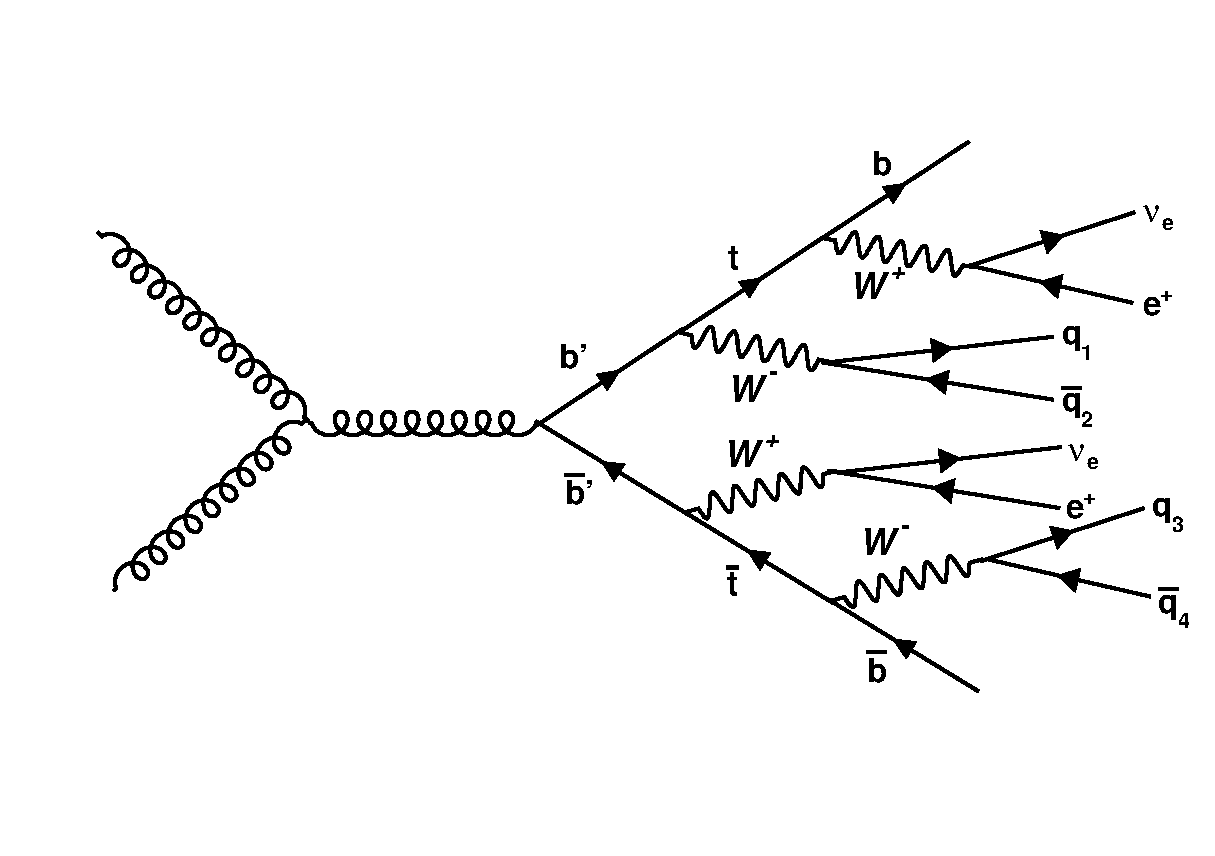
\includegraphics[scale=0.30]{figures/samesign/Feyn-bprime}}
\subfigure[\label{feynman_t53pair}]{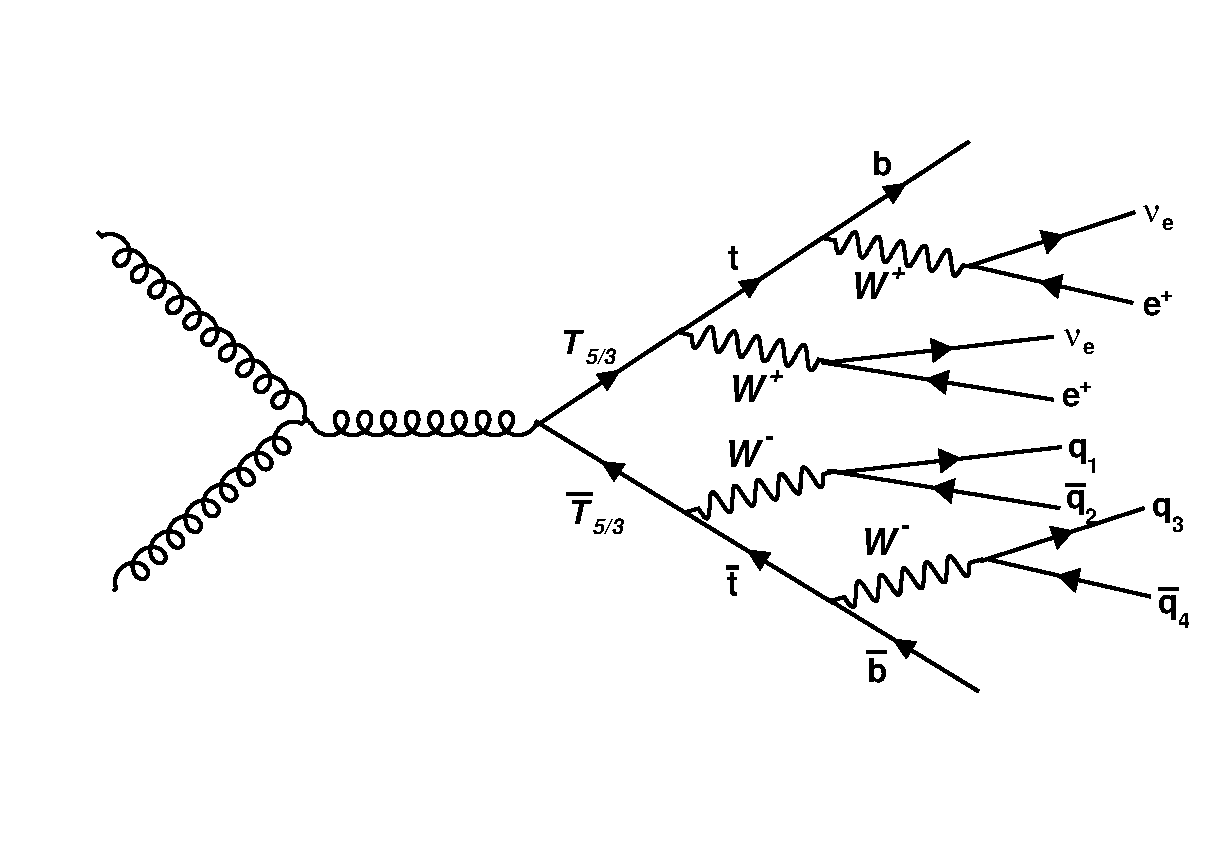
\includegraphics[scale=0.30]{figures/samesign/Feyn-T53pair}}
\subfigure[\label{feynman_t53single}]{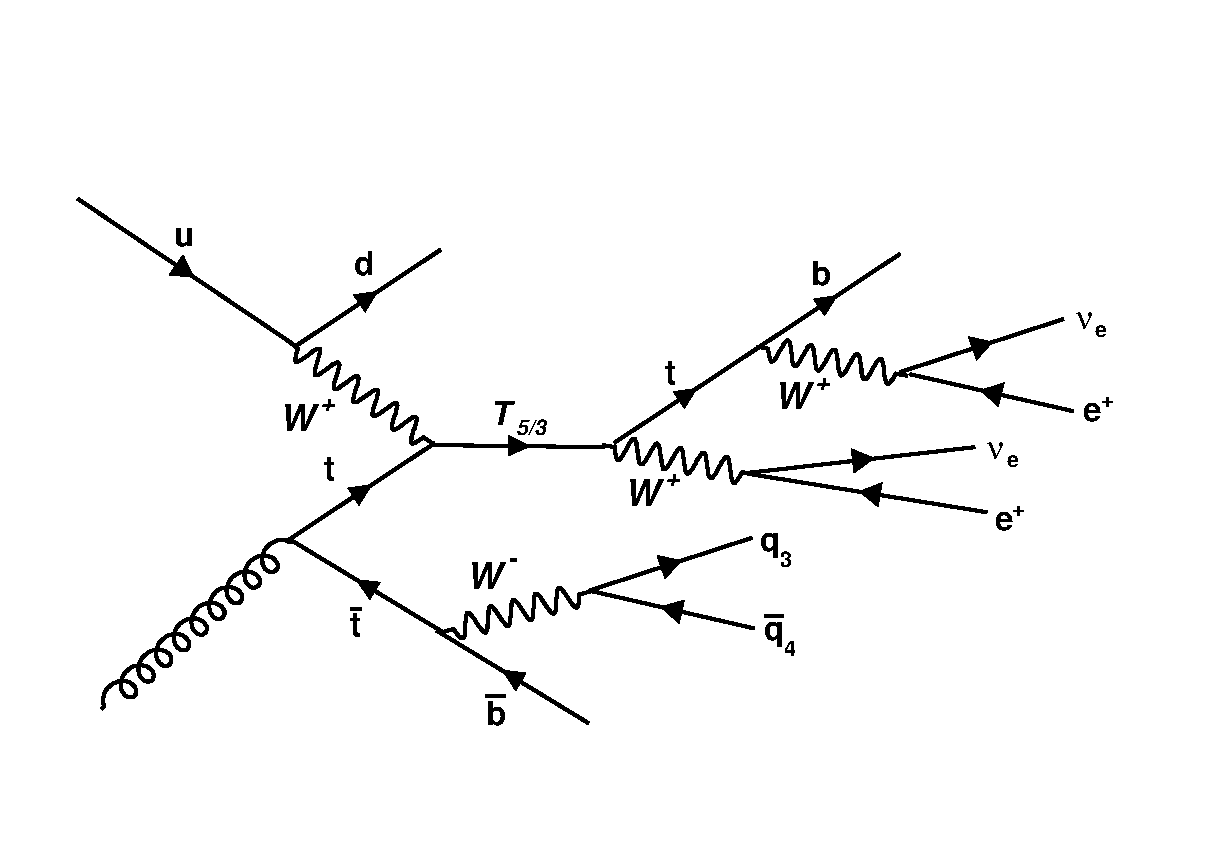
\includegraphics[scale=0.30]{figures/samesign/Feyn-T53single}}
\subfigure[\label{feynman_4t}]{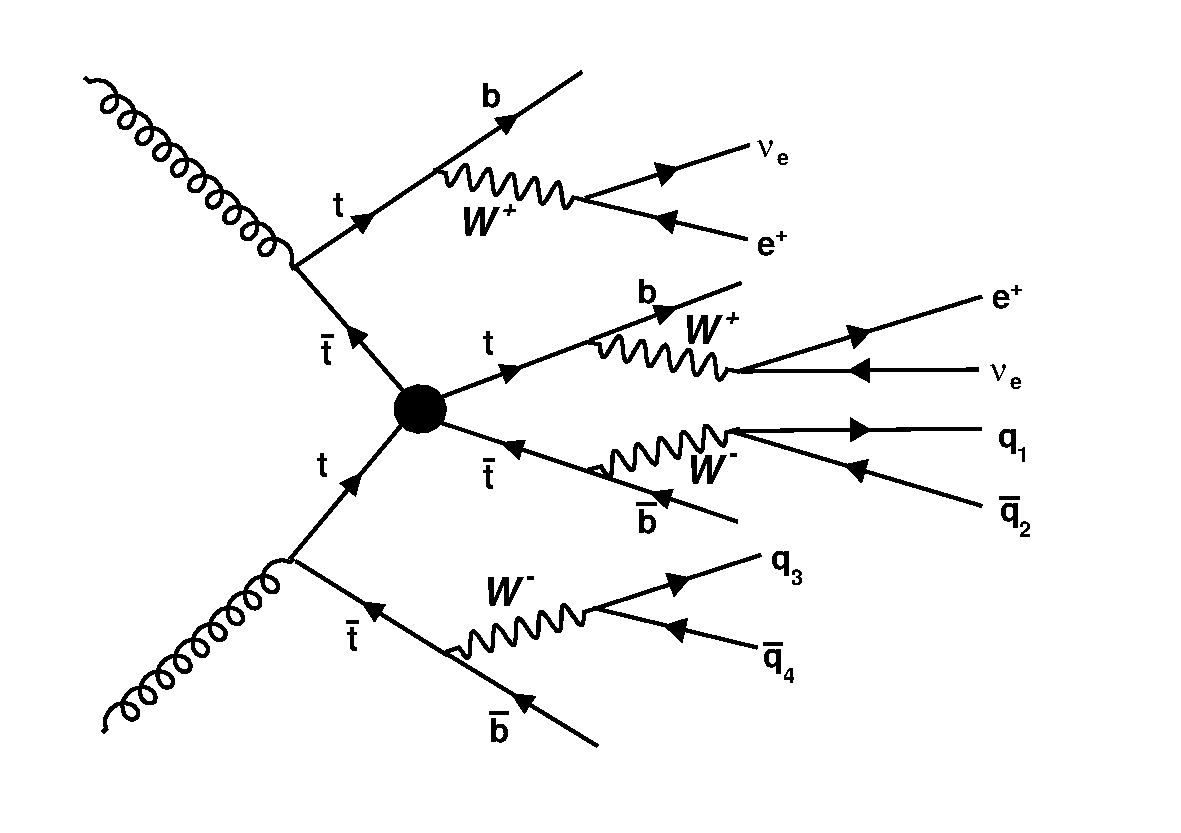
\includegraphics[scale=0.30]{figures/samesign/Feyn-4t}}
\caption{Examples of Feynman diagrams for $b^\prime$ pair production (a), $T_{5/3}$ pair (b) and
single (c) productions, and four top quarks event production through a four-top quark contact interaction (d).}
\end{figure}


\section{Pair production of down-type heavy quarks ($b^\prime$)}

The first model considered in this section proposes an extension to the standard model that includes a fourth generation of down-type heavy quarks, which we will here refer to as $b^\prime$~\cite{Holdom:2006mr}.
The discovery of the higgs boson and the measurement of its production cross-section have put constraints on on models proposing fourth generation quarks.
Direct Higgs searches combining the search channels $\gamma \gamma$, $ZZ$, $WW$, $b\bar{b}$, and $\tau^{+} \tau^{-}$ disfavor a sequential fourth generation~\cite{Eberhardt:2012gv,Djouadi:2012ae,Eberhardt:2012sb,Eberhardt:2012ck} as the model predicts specific ratios of branching ratios into final states which are not supported by the experimental results.
Specifically, Higgs production cross section in gluon-gluon fusion at the LHC is enhanced by about a factor of nine for a Higgs boson mass of 126 GeV, but associated Higgs production ($HW$ and $HZ$) relevant for searching for $H \rightarrow b\bar{b}$ does not get such an enhancement factor from the presence of fourth generation.
However, when including a fourth generation model, the Higgs decay branching fraction to $\gamma \gamma$ is heavily suppressed, which can compensate for the enhancement to the gluon-gluon production mode.
More generally, numerious non-Standard Higgs scenerios can significantly alter production cross-sections and Higgs branching ratios.
For example, a fourth generation extension might still be in accordance with experimental constraints when extending the Higgs sector, as described in Two-Higgs-Doublet models~\cite{BarShalom:2012ms}. 
Therefore, it remains desirable to perform direct searches for fourth-generation quarks.

%% \section{Pair production of down-type heavy quarks ($b^\prime$)}
%% The first signal process is based on the hypothesis that a fourth
%% generation of fermions may extend the particle content of the
%% SM~\cite{Holdom:2006mr}. Direct Higgs searches combining the search
%% channels $\gamma \gamma$, $ZZ$, $WW$, $b\bar{b}$, and $\tau^{+}
%% \tau^{-}$ disfavor a sequential fourth
%% generation~\cite{Eberhardt:2012gv,Djouadi:2012ae,Eberhardt:2012sb,Eberhardt:2012ck}
%% as the model predicts a specific hierarchy of signal strengths which
%% is not supported by the experimental results: while Higgs production
%% cross section in gluon-gluon fusion at the Tevatron and LHC is
%% enhanced by about a factor of nine for a Higgs boson mass of 126 GeV,
%% associated Higgs production ($HW$ and $HZ$) relevant for searching for
%% $H \rightarrow b\bar{b}$ does not get such an enhancement factor from
%% the presence of fourth generation. However, the Higgs decay branching fraction
%% to $\gamma \gamma$ is heavily suppressed in a sequential fourth
%% generation model and can even over-compensate the gluon-gluon fusion
%% enhancement factor. Moreover, all Higgs branching fractions can be suppressed by
%% a common reduction factor by adjusting the heavy neutrino mass of the
%% fourth generation Dirac neutrino so that invisible Higgs decays become
%% possible. Additionally a fourth generation extension might still be in accordance
%% with experimental constraints when extending the Higgs sector, like in
%% Two-Higgs-Doublet models~\cite{BarShalom:2012ms}.

In the scenerio studied in this section, the $b^\prime$ is not allowed to decay into a $t^\prime$, but rather is limited to decaying to$u/c+W^{-}$ as well as $t+W^{-}$, as long as $m_{b^\prime}-m_{t}> m_W$, which is equivalent to $m_{b^\prime} > 255 \GeV{}$.

Although not completely excluding $m_{t^\prime}<m_{b^\prime}$, electroweak precision observables favour the region $m_{t^\prime}>m_{b^\prime}$, and differences in mass as large as $m_{t^\prime}-m_{b^\prime}=m_{W}$ are very much disfavoured. 
Assuming $V_{u(c) b^\prime}\ll V_{t b^\prime}$, the dominant decay is $b^\prime \rightarrow t+ W^{-}$.
This results in decay states as seen in Figure~\ref{feynman_bprime}, for which a search involving pairs of same-sign charged leptons is well motivated.

%% Electroweak precision observables favour the region $m_{t^\prime}>m_{b^\prime}$ 
%% (although $m_{t^\prime}<m_{b^\prime}$ is not excluded), with differences as large 
%% as $m_{t^\prime}-m_{b^\prime}=m_{W}$ being disfavoured. In the scenario studied in this
%% note, the $b^\prime$ can not decay into a $t^\prime$ and decays into the 
%% final states $u/c+W^{-}$ as well as $t+W^{-}$, as long as $m_{b^\prime}-m_{t}> m_W$, which is equivalent 
%% to $m_{b^\prime} > 255 \GeV{}$. If one assumes $V_{u(c) b^\prime}\ll V_{t b^\prime}$ the dominant decay is 
%% $b^\prime \rightarrow t+ W^{-}$. In this case it is possible to search for $b^\prime$ 
%% quarks by looking for pairs of same-sign charged leptons accompanied by a large number of jets,
%% two of them arising from $b$ quarks, as illustrated in Figure~\ref{feynman_bprime}.

\section{Single and pair production of heavy top quark partners ($T_{5/3}$)}

A natural, non-supersymmetric solution to the hierarchy problem involves modeling the Higgs as a pseudo-Goldstone boson~\cite{Contino:2008hi}
This model requires the inclusion of heavy, fermionic partners to the top quark which couple to the Standard Model through a $W$ boson, preferentially to the third generation.
We here search for the production of these top parners with electric charge charge $Q_{e}=5/3$, which we denoted as $T_{5/3}$, through either single-production or pair-production mechanisms.
The pair-production of $T_{5/3}$ particles is, to lowest order, kinematically equivalant to the pair-production of $b^{\prime}$ quarks, and therefore the production cross-sections are nearly identical as a function of mass.
The cross-section of single-production of $T_{5/3}$ depends on the coupling constant of the t$WT_{5/3}$ vertex, which we denote as $\lambda$.
In this analysis, we study the cases $\lambda=1$, $\lambda=3$ and $\lambda\ll 1$, where in the latter case, the single-production mode vanishes.
The contribution of other top partners described in ~\cite{Contino:2008hi}, such as $T_{2/3} \rightarrow Zt$, would slightly increase the expected number of expected signal events, but these contributions are not taken into account in this analysis. 

%% \section{Single and pair production of heavy top quark partners ($T_{5/3}$)}
%% The second signal process is based on a model where the Higgs is a pseudo-Goldstone 
%% boson~\cite{Contino:2008hi}. This natural, non-supersymmetric solution to the hierarchy 
%% problem requires fermionic partners of the top quark. 
%% These heavy fermions are coupled to the SM quarks through a $W$ boson,
%% preferentially to the third generation.
%% We study here the pair (Figure~\ref{feynman_t53pair}) and single (Figure~\ref{feynman_t53single}) 
%% productions of the top partners with electric charge $Q_{e}=5/3$, denoted $T_{5/3}$. It must be
%% noted that the pair production is kinematically equivalent to the pair production
%% of $b^\prime$ heavy quarks, and therefore the production cross sections are the same
%% for a given $b^\prime$ or $T_{5/3}$ mass. For the single production, the production 
%% cross section depends on the coupling constant $\lambda$ of the t$WT_{5/3}$ vertex.
%% In this analysis, we study the cases $\lambda=1$, $\lambda=3$ and $\lambda\ll 1$. In the
%% latter case, the single production vanishes and the study corresponds to the pair production
%% of $b^\prime$ quarks. 
%% Other top partners predicted in~\cite{Contino:2008hi}, such as $T_{2/3} \rightarrow Zt$, would slightly 
%% increase the number of expected signal events. Their contribution has
%% not been taken into account here.

\section{Production of events containing four top quarks}

Another, more generic signal process being studied is the production of events containing a four right-handed top quark contact interaction vertex ($t\bar{t}t\bar{t}$), known simply as the four tops signal, which is described in Ref.~\cite{Degrande:2010kt}.
Only the contact interaction operator with right-handed top quarks is considered, as left-handed top operators are already strongly constrained by electroweak precision data \cite{PhysRevD.51.3888}.

The signal is motivated by te many new physics models that couple strongly to the top quark, including interactions related to electroweak symmetry breaking, models with a composite top quark, or models with new colored, heavy particles that decay preferentially into top quarks.
These models can produce events containing four top-quarks at a much higher rate than the Standard Model, which predicts a four-tops cross-section on the order of 1~fb at 7~\TeV.
Searches for a four-tops signal are sensitive to new physics phenomena which do not affect $t\bar{t}$ production, for which no deviation from the SM expectations has been observed so far.
This analysis therefore does not aim at testing a particular theory but rather a class of theories where new physics manifests itself at low energy as a four right-handed top contact interaction. 
This is the case for theories predicting new heavy vector particles strongly coupled to the right-handed top quark such as top compositeness~\cite{PhysRevD.78.074026,1126-6708-2008-04-087,1126-6708-2009-05-022} or Randall-Sundrum theories~\cite{Guchait:2007jd}.

%% \section{Production of events containing four top quarks}
%% The third and last signal process is the production of events containing four top quarks ($t\bar{t}t\bar{t}$). 
%% Indeed, many new physics models couple strongly to the top quark, including a new interaction 
%% related to electroweak symmetry breaking that couples uniquely to the top quark,
%% models where only the top quark is composite, 
%% or new coloured heavy particles that decay preferentially
%% to top quarks. Many of these new physics models predict an enhanced rate
%% of events containing four top quarks with respect to the SM production, which is of the order of 1~fb 
%% at 7~\TeV. Therefore, searching for events containing four top quarks could open
%% a window on new physics phenomena which do not affect $t\bar{t}$ production, for which
%% no deviation from the SM expectations has been observed so far.

%% This analysis follows the approach described in Ref.~\cite{Degrande:2010kt}, which consists of searching 
%% for the experimental signature of a four right-handed top quark contact interaction 
%% (Figure~\ref{feynman_4t}). Only the contact interaction operator with right-handed top quarks 
%% is considered, as left-handed top operators are already strongly constrained by electroweak precision 
%% data \cite{PhysRevD.51.3888}. This analysis therefore does not aim at testing a particular theory 
%% but rather a class of theories where new physics manifests itself at low energy as a four right-handed 
%% top contact interaction. This is the case for theories predicting new heavy vector particles strongly 
%% coupled to the right-handed top quark such as top 
%% compositeness~\cite{PhysRevD.78.074026,1126-6708-2008-04-087,1126-6708-2009-05-022} or 
%% Randall-Sundrum theories~\cite{Guchait:2007jd}.


\section{Analysis Strategy}\label{sect:strategy}

The exotic signals described in this section share several kinematic features in common which can be used to select those events with a high efficiency while rejecting a large amount of Standard Model backgrounds.
The most important of these features is the presence of multiple leptons, including a pair of same-sign leptons.
In addition, because these exotic signals involve the production of heavy particles, the final decay products will tend to have significant transverse momentum, which leads to a high distribution of $HT$ (the scalar sum of the transverse momentum of reconstructed and selected objects) in signal events.
The decays of top quarks results in neutrinos in the final state, which leads to a high distribution of missing transverse momentum, as well as b-quarks, which result in b-jets that can be tagged for further background rejection.

These properties were studied extensively in using Monte Carlo simulation of signal and background events.
Because the expected level of background from the standard model was expected to be small, a cut-and-count measurement strategy was decided upon, when a number of orthogonal signal regions are defined and the number of measured events passing that signal selection of each individual region is compared to the expected amount of signal and background events in those regions.
Separate signal regions were constructed for final states that result in two electrons ($ee$), two muons ($\mu \mu$), or an electron and a muon ($e \mu$).
The selection of the signal regions was defined using detailed numeric optimizations, where the threshold cuts on several kinematic variables were tuned to maximize the expected significance in each signal region individually.
Since the background levels vary across the three signal regions, each the selections were optimized individually in each signal region.
The results obtained in each signal region were then combined using a simultaneous likelihood describing all signal regions, including their backgrounds and systematic uncertainties.
For each model analyzed, the final limits shown were evaluated using this simultaneous likelihood


\section{Object reconstruction}\label{sect:objects}

The signal region event selection was based on definitions of final state physical objects that are consistent across all three selection channels.
These object definitions conform to the central recommendations of various performance groups within the ATLAS experiment, and match the definitions of the Top Group at the time the analysis was performed.
These definitions can be thought of as a mapping from the detector's electronic response to a $pp$ collision to a logical set of electrons, muons, jets, b-jets, and primary vertices.
Primary vertices are defined as the single vertex in an event with the highest summed track $\pT^2$, where each track entering that quantity must have $\pT>0.4 \GeV{}$.

%% \section{Object reconstruction}\label{sect:objects}
%% From the various signals recorded in the ATLAS detector after the $pp$ collision, we reconstruct
%% physics objects that are candidates for jets, electrons and muons. The primary vertex is defined
%% as the vertex with the highest summed track $\pT^2$, each having $\pT>0.4 \GeV{}$.

Selected electrons are chose from showers in the electromagnetic calorimeter which have a good quality track pointing to the calorimeter cluster.
Electrons are required to have $\ET>25 \GeV$ and are further selected as passing a ``tight'' identification requirement, which is based on a number of variables describing the details of the shape of the electromagnetic cluster and the quality of its associated track~\cite{Aad:2011mk}.
The candidate electron is required to fall inside a well instrumented region of the detector ($|\eta_\mathrm{cluster}|<2.47$, excluding $1.37<|\eta_\mathrm{cluster}|<1.52$).
The electron must be isolated from tracks and calorimeter clusters not associated with the electron, and so isolation cuts are imposed on the transverse energy in a cone of $\Delta R = 0.2$ around the electron ($\ET^{\Delta R=0.2}$) and on the total transverse momentum of all tracks within $\Delta R = 0.3$ of the electron ($\pT^{\Delta R=0.3}$).
These cuts are chosen to have 90\% efficiency on real, high-pt electrons.
In addition, electrons are required to be isolated from selected jets (to be defined below) by requiring $\Delta R(e,\mathrm{jet})>0.4$. 

%% Electrons are required to have a shower shape in the electromagnetic calorimeter consistent with
%% expectation, as well as a good quality track pointing to the cluster in the calorimeter.
%% Candidate electrons with transverse energy $\ET>25 \GeV$ are required to pass the ``tight''
%% ATLAS electron quality cuts~\cite{Aad:2011mk}, and to fall inside a well instrumented region
%% of the detector ($|\eta_\mathrm{cluster}|<2.47$, excluding $1.37<|\eta_\mathrm{cluster}|<1.52$). 
%% In addition, \ET{} and $\eta_\mathrm{cluster}$ dependent isolation cuts are imposed on the transverse 
%% energy in a cone of $\Delta R = 0.2$ around the electron ($\ET^{\Delta R=0.2}$) and on the total 
%% transverse momentum of all tracks within $\Delta R = 0.3$ of the electron ($\pT^{\Delta R=0.3}$).
%% The cuts are chosen such that the efficiency of each isolation requirement is 90\%. The values used
%% in the cuts range from 1.4~\GeV{} to 3.7~\GeV{} for $\ET^{\Delta R=0.2}$ and from 1~\GeV{} to 1.05~\GeV{}
%% for $\pT^{\Delta R=0.3}$. Electrons are also required to be well 
%% isolated from jets ($\Delta R(e,\mathrm{jet})>0.4$).

A set of candidate jets are is defined using the anti-$k_t$~\cite{Cacciari:2008gp} algorithm with a distance parameter of 0.4.
From this set, selected jets are defined by further requiring that they have $\pt>25 \GeV$ and $|\eta|<2.5$.
The energy used for this requirement is calibrated to the hadronic energy scale using $\pt$- and $\eta$-dependent corrections derived from collision and test-beam data as well as simulation~\cite{Aad:2011he}.
To separate jets originating from the primary vertex from those coming from pileup, a cut on a quantity called the jet-vertex-fraction (JVF) is used.
The jet-vertex-fraction considers all tracks of a particular jet that have $\pt>0.4~\GeV{}$.
It is defined as the ratio of the sum of $\pt$ of all tracks for that jet which originate from primary vertex over the sum of the $\pt$ of all tracks matched to the jet. 
Jets with associated tracks are required to have $JVF>0.75$, but jets without any associated tracks are accepted as well.
In order to prevent double-counting of clusters that are associated with selected electrons as jets, selected jets are required to be separated from selected electrons (as defined above) by requiring $\Delta R(\mathrm{jet},e) > 0.2$.

%% Jets are reconstucted in the calorimeter using the anti-$k_t$~\cite{Cacciari:2008gp} algorithm with
%% a distance parameter of 0.4. Jets are required to satisfy $\pt>25 \GeV$ and $|\eta|<2.5$. They are
%% calibrated to the hadronic energy scale using $\pt$- and $\eta$-dependent corrections derived from
%% collision and test-beam data as well as simulation~\cite{Aad:2011he}. To reject jets from pileup, 
%% a quantity called jet-vertex-fraction, $JVF$, is defined as the ratio of the sum
%% of the $\pt$ of all tracks, with $\pt>0.4~\GeV{}$, within the jet that originate from the primary 
%% vertex associated to the hard-scattering collision, over the sum of the $\pt$ of all tracks 
%% matched to the jet. Jets with associated tracks are required to have $JVF>0.75$; we also
%% accept jets without any associated tracks. In order to avoid reconstructing electrons as jets,
%% the latter are required to have an angular separation 
%% $\Delta R(\mathrm{jet},e)$\footnote{$\Delta R=\sqrt{\Delta\eta^2+\Delta\phi^2}$ is the distance 
%% between two objects, in
%% the plane $\eta-\phi$, where $\eta$ is the pseudo-rapidity and $\phi$ the angle in the transverse
%% plane.} of at least 0.2.

Jets associated with a b-quark, known as b-jets, are further chosen from the set of selected jets by using a $b$-tagging algorithm~\cite{ATLAS-CONF-2012-043} at an operating point of 70\% efficiency for $b$-jets, which corresponds to a mis-tag rate of less than 1\%, as determined in simulated $t\bar{t}$ events.

%% Jets from the decay of heavy flavor hadrons are selected by a multivariate $b$-tagging 
%% algorithm~\cite{ATLAS-CONF-2012-043} at an operating point of 70\% efficiency for $b$-jets, which
%% corresponds to a
%% mis-tag rate of less than 1\%, as determined in simulated $t\bar{t}$ events.

Muons are selected by combining tracks from the Muon Spectrometer and the inner detector, and the combined track is required to have $\pt>20 \GeV$.
Muons fall within an angle of $|\eta|<2.5$ and must pass a number of quality cuts defined by ATLAS performance groups.
In additon, muons are required to be isolated by requiring the transverse energy within a cone of $\Delta R = 0.2$ to be $<4\GeV{}$ and the total transverse momentum of all tracks within $\Delta R = 0.3$ to be $<2.5~\GeV{}$.
Muons must isolated from jets, which is imposed by requiring $\Delta R(\mu,\mathrm{jet})>0.4$.
A cut attempting to reject muons originating from cosmic rays rejects muons passing through the center of the detector and having an angle between them > 3.1~rad.
Events where a selected electron shares a track with a selected muon are rejected.

%% Muons are required to have transverse momentum $\pt>20 \GeV$, to pass standard ATLAS muon quality
%% cuts~\cite{ATLAS-CONF-2011-063}, to be well measured in both the inner detector and the muon 
%% spectrometer and to fall within $|\eta|<2.5$. In addition, isolation cuts require the transverse energy 
%% within a cone of $\Delta R = 0.2$ and the total transverse momentum of all tracks within $\Delta R = 0.3$
%% of the muon candidate to be less than 4~\GeV{} and 2.5~\GeV{}, respectively. 
%% Muons are also required to be well isolated from jets ($\Delta R(\mu,\mathrm{jet})>0.4$).
%% Events that contain two muons which could originate from a cosmic muon passing
%% through the center of the detector are rejected, when the angle between them in the transverse plane
%% is larger than 3.1~rad. Events are also rejected if there is a candidate electron that shares a track
%% with a candidate muon.

The missing transverse momentum (\met{}) is calculated using the calorimeter clusters and corrected using the set of selected electrons, muons and jets~\cite{Aad:2012re}.


%% The missing transverse momentum (denoted \met{}) is calculated using calorimeter clusters and corrected
%% for the presence of electrons, muons and jets~\cite{Aad:2012re}.

\section{Event selection}\label{sect:selection}

Using the objects as defined above, three signal regions are defined, which correspond to $ee$, $e \mu$, and $\mu \mu$ final states.

All events used in the analysis are required to have a primary vertex determined using at least five tracks.
Events in the signal region are selected with the following criteria:
\begin{itemize}
\item Events must contain at least two selected of the same charge. 
\item The leading lepton in the pair must have \pT $>25$ \GeV{}.
\item At least one of the selected leptons must match the one that triggered the readout of the event.
\item Events must contain at least two jets, including at least one $b$-tagged jet.
\item In the $ee$ or $\mu\mu$ channel, the invariant mass of the two selected leptons must exceed 15 \GeV{} and be out of the $Z$-boson mass window; i.e. $|m_{\ell\ell} - m_Z| > 10 \GeV$.
\item The \met{} must be greater than 40 \GeV{}.
\item The $\HT{}$, defined as the scalar sum of the $\pt$ of all leptons and jets, must exceed 550 $\GeV{}$.
\end{itemize}
The category of each event is determined by the type of leptons used in the selected same-sign pair.
In events with more than one same-sign pair, the pairs are sorted according to the leading lepton \pT, then by the subleading lepton \pT, and the first pair is used to categorize the event.
These selection criteria are the result of an optimization, performed separately for the three different signals, varying the requirements on \HT{}, on the number of jets and on the number of $b$-jets.

The final acceptance for the different signals is shown in Table~\ref{effsignal}.
The expected number of events for the different signals after applying this event selection, rescaled to the integrated luminosity of the recorded data, is summarized in Table~\ref{yieldsignal}.

\begin{table}[p]
  \begin{center}
    \caption{Signal acceptance (in percent) of the signal region selection. The acceptance is calculated 
      with respect to the full signal production including all decay modes of the $W$ bosons.}\label{effsignal}
    \begin{tabular}{c|c|c|c|c|c|c|c|c|c|c|c}
      \hline\hline
      Mass [GeV] & 300 & 350 & 400 & 450 & 500 & 550 & 600 & 650 & 700 & 750 & 800 \\
      \hline
      \multicolumn{12}{c}{$b^\prime$ / $T_{5/3}$ pair production $\lambda\ll1$} \\
      \hline
      $ee$ & 0.04 & 0.11 & 0.18 & 0.26 & 0.30 & 0.35 & 0.41 & 0.40 & 0.41 & 0.45 & 0.43 \\
      $e\mu$ & 0.20 & 0.42 & 0.62 & 0.83 & 1.02 & 1.09 & 1.17 & 1.27 & 1.34 & 1.33 & 1.31 \\
      $\mu\mu$ & 0.16 & 0.24 & 0.43 & 0.52 & 0.63 & 0.78 & 0.76 & 0.83 & 0.84 & 0.83 & 0.84 \\
      \hline
      \multicolumn{12}{c}{$T_{5/3}$ single production only $\lambda=1$} \\
      \hline
      $ee$ & & & & 0.04 & & 0.05 & & 0.09 & & 0.10 & \\
      $e\mu$ & & & & 0.14 & & 0.18 & & 0.26 & & 0.28 & \\
      $\mu\mu$ & & & & 0.07 & & 0.11 & & 0.14 & & 0.16 & \\
      \hline
      \multicolumn{12}{c}{$T_{5/3}$ single production only $\lambda=3$} \\
      \hline
      $ee$ & & & & 0.04 & & 0.06 & & 0.08 & & 0.11 & \\
      $e\mu$ & & & & 0.13 & & 0.17 & & 0.22 & & 0.26 & \\
      $\mu\mu$ & & & & 0.09 & & 0.10 & & 0.14 & & 0.17 & \\
      \hline
      \multicolumn{12}{c}{Four top quarks event production} \\
      \hline
      $ee$ & \multicolumn{11}{c}{0.23} \\
      $e\mu$ & \multicolumn{11}{c}{0.81} \\
      $\mu\mu$ & \multicolumn{11}{c}{0.58} \\
      \hline
    \end{tabular}

    \vspace{5mm}
 
    \caption{Expected number of selected events with Monte Carlo statistical uncertainties 
      for the different signals, for an integrated luminosity of 4.7~\ifb{}.}\label{yieldsignal}
    \begin{tabular}{c|c|c|c|c}
      \hline\hline
      \multicolumn{2}{c|}{Signal parameter}  & \multicolumn{3}{c}{Channel} \\
      \hline
      Coupling& Mass [\GeV{}]      & $ee$ & $e\mu$ & $\mu\mu$ \\ 
      \hline
       \multicolumn{5}{c}{$b^\prime$ / $T_{5/3}$ pair production} \\
      \hline
      & 300 & $16.8 \pm 2.2$   & $77.8 \pm 5.0$   & $57.8 \pm 4.3$     \\ 
      & 350 & $16.8 \pm 1.4$   & $64.5 \pm 2.9$   & $36.2 \pm 2.2$     \\ 
      & 400 & $12.3 \pm 0.8$   & $41.9 \pm 1.5$   & $28.2 \pm 1.3$     \\ 
      & 450 & $8.05 \pm 0.46$   & $26.18 \pm 0.85$   & $16.25 \pm 0.66$     \\ 
      & 500 & $4.72 \pm 0.20$   & $15.84 \pm 0.38$   & $9.71 \pm 0.30$     \\ 
      $\lambda\ll1$ & 550 & $2.83 \pm 0.14$   & $8.88 \pm 0.25$   & $6.34 \pm 0.22$     \\ 
      & 600 & $1.78 \pm 0.08$   & $5.09 \pm 0.14$   & $3.29 \pm 0.11$     \\ 
      & 650 & $0.98 \pm 0.04$   & $3.06 \pm 0.08$   & $2.00 \pm 0.07$     \\ 
      & 700 & $0.57 \pm 0.03$   & $1.84 \pm 0.05$   & $1.15 \pm 0.04$     \\ 
      & 750 & $0.36 \pm 0.02$   & $1.07 \pm 0.03$   & $0.66 \pm 0.02$     \\ 
      & 800 & $0.20 \pm 0.01$   & $0.61 \pm 0.02$   & $0.39 \pm 0.01$     \\ 
      \hline
      \multicolumn{5}{c}{$T_{5/3}$ single and pair production} \\
      \hline
      & 450 & $8.82 \pm 0.46$ & $28.73 \pm 0.86$ & $17.54 \pm 0.67$ \\
      $\lambda=1$ & 550 & $2.87 \pm 0.14$ & $9.04  \pm 0.25$ & $6.44  \pm 0.22$ \\
      & 650 & $1.02 \pm 0.04$ & $3.17  \pm 0.08$ & $2.06  \pm 0.07$ \\
      & 750 & $0.38 \pm 0.02$ & $1.13  \pm 0.03$ & $0.70  \pm 0.02$ \\
      \hline
      & 450 & $8.77 \pm 0.46$ & $28.31 \pm 0.86$ & $17.71 \pm 0.67$ \\
      $\lambda=3$ & 550 & $3.29 \pm 0.14$ & $10.16  \pm 0.26$ & $7.14  \pm 0.22$ \\
      & 650 & $1.28 \pm 0.05$ & $3.89  \pm 0.09$ & $2.53  \pm 0.07$ \\
      & 750 & $0.57 \pm 0.02$ & $1.55  \pm 0.03$ & $0.98  \pm 0.03$ \\
      \hline
      \multicolumn{5}{c}{Four top quarks event production} \\
      \hline
      \multicolumn{2}{c|}{$\sigma=12.6$~fb} & $0.138 \pm 0.010$ & $0.483\pm 0.019$& $0.343\pm 0.015$\\
      \hline
    \end{tabular}
  \end{center}
\end{table}


%% \section{Event selection}\label{sect:selection}
%% All events used in the analysis are required to have a primary vertex
%% determined from at least five tracks.
%% Events in the signal region are selected with the following criteria:
%% \begin{itemize}
%% \item Events must contain at least two isolated leptons of the same charge. In events with more than one
%%   same-sign pair, the pairs are sorted according to the leading lepton
%%   \pT, then by the subleading lepton \pT. The first pair is chosen. An additional cut
%%   is performed on the leading lepton of the pair, requiring it to have \pT\ $>25$ \GeV{}. At this
%%   stage, each event is categorized as being a $ee$, $e\mu$ or $\mu\mu$ candidate, depending on the
%%   selected lepton flavors. At least one of the selected leptons must match the one that triggered
%%   the readout of the event.
%% \item Events must contain at least two jets, including at least one $b$-tagged jet.
%% \item In the $ee$ or $\mu\mu$ channel, the invariant mass of the two selected leptons must exceed 15 \GeV{} and be out of the $Z$-boson mass window; i.e. $|m_{\ell\ell} - m_Z| > 10 \GeV$.
%% \item The \met{} must be greater than 40 \GeV{}.
%% \item The \HT{}, defined as the scalar sum of the \pt\  of all leptons and jets, must exceed 550 \GeV{}.
%% \end{itemize}
%% These selection criteria are the result of an optimization, performed separately for the three different
%% signals, varying the requirements on \HT{}, on the number of jets and on the number of $b$-jets.
%% Finally, a common selection has been defined. The final acceptance for the different
%% signals is shown in Table~\ref{effsignal}.

% \begin{table}[t]
%   \begin{center}
%     \caption{Signal acceptance (in percent) of the signal region selection. The acceptance are calculated
%       with respect to the full production, without any requirement on the number of 
%       leptons.}\label{effsignal}
%     \begin{tabular}{c|c|c|c|c}
%       \hline\hline
%       \multicolumn{2}{c|}{Signal parameter}  & \multicolumn{3}{c}{Channel} \\
%       \hline
%       Coupling $\lambda$ & Mass [\GeV{}]      & $ee$ & $e\mu$ & $\mu\mu$ \\ 
%       \hline
%        \multicolumn{5}{c}{$b^\prime$ / $T_{5/3}$ pair production} \\
%       \hline
%       & 300 & $0.04$   & $0.20$   & $0.16$     \\ 
%       & 350 & $0.11$   & $0.42$   & $0.24$     \\ 
%       & 400 & $0.18$   & $0.62$   & $0.43$     \\ 
%       & 450 & $0.26$   & $0.83$   & $0.52$     \\ 
%       & 500 & $0.30$   & $1.02$   & $0.63$     \\ 
%       $\ll1$ & 550 & $0.35$   & $1.09$   & $0.78$     \\ 
%       & 600 & $0.41$   & $1.17$   & $0.76$     \\ 
%       & 650 & $0.40$   & $1.27$   & $0.83$     \\ 
%       & 700 & $0.41$   & $1.34$   & $0.84$     \\ 
%       & 750 & $0.45$   & $1.33$   & $0.83$     \\ 
%       & 800 & $0.43$   & $1.31$   & $0.84$     \\ 
%       \hline
%       \multicolumn{5}{c}{$T_{5/3}$ single production only} \\
%       \hline
%       & 450 & $0.04$ & $0.14$ & $0.07$ \\
%       1 & 550 & $0.05$ & $0.18$ & $0.11$ \\
%       & 650 & $0.09$ & $0.26$ & $0.14$ \\
%       & 750 & $0.10$ & $0.28$ & $0.16$ \\
%       \hline
%       & 450 & $0.04$ & $0.13$ & $0.09$ \\
%       3 & 550 & $0.06$ & $0.17$ & $0.10$ \\
%       & 650 & $0.08$ & $0.22$ & $0.14$ \\
%       & 750 & $0.11$ & $0.26$ & $0.17$ \\
%       \hline
%       \multicolumn{5}{c}{Four top quarks event production} \\
%       \hline
%       \multicolumn{2}{c|}{} & $0.23$ & $0.81$& $0.58$\\
%       \hline
%     \end{tabular}
%  \end{center}
% \end{table}

%% The expected number of events for the different signals after applying this event selection, rescaled to
%% the integrated luminosity of the recorded data, is summarized in Table~\ref{yieldsignal}.

%% \begin{table}[p]
%%   \begin{center}
%%     \caption{Signal acceptance (in percent) of the signal region selection. The acceptance is calculated 
%%       with respect to the full signal production including all decay modes of the $W$ bosons.}\label{effsignal}
%%     \begin{tabular}{c|c|c|c|c|c|c|c|c|c|c|c}
%%       \hline\hline
%%       Mass [GeV] & 300 & 350 & 400 & 450 & 500 & 550 & 600 & 650 & 700 & 750 & 800 \\
%%       \hline
%%       \multicolumn{12}{c}{$b^\prime$ / $T_{5/3}$ pair production $\lambda\ll1$} \\
%%       \hline
%%       $ee$ & 0.04 & 0.11 & 0.18 & 0.26 & 0.30 & 0.35 & 0.41 & 0.40 & 0.41 & 0.45 & 0.43 \\
%%       $e\mu$ & 0.20 & 0.42 & 0.62 & 0.83 & 1.02 & 1.09 & 1.17 & 1.27 & 1.34 & 1.33 & 1.31 \\
%%       $\mu\mu$ & 0.16 & 0.24 & 0.43 & 0.52 & 0.63 & 0.78 & 0.76 & 0.83 & 0.84 & 0.83 & 0.84 \\
%%       \hline
%%       \multicolumn{12}{c}{$T_{5/3}$ single production only $\lambda=1$} \\
%%       \hline
%%       $ee$ & & & & 0.04 & & 0.05 & & 0.09 & & 0.10 & \\
%%       $e\mu$ & & & & 0.14 & & 0.18 & & 0.26 & & 0.28 & \\
%%       $\mu\mu$ & & & & 0.07 & & 0.11 & & 0.14 & & 0.16 & \\
%%       \hline
%%       \multicolumn{12}{c}{$T_{5/3}$ single production only $\lambda=3$} \\
%%       \hline
%%       $ee$ & & & & 0.04 & & 0.06 & & 0.08 & & 0.11 & \\
%%       $e\mu$ & & & & 0.13 & & 0.17 & & 0.22 & & 0.26 & \\
%%       $\mu\mu$ & & & & 0.09 & & 0.10 & & 0.14 & & 0.17 & \\
%%       \hline
%%       \multicolumn{12}{c}{Four top quarks event production} \\
%%       \hline
%%       $ee$ & \multicolumn{11}{c}{0.23} \\
%%       $e\mu$ & \multicolumn{11}{c}{0.81} \\
%%       $\mu\mu$ & \multicolumn{11}{c}{0.58} \\
%%       \hline
%%     \end{tabular}

%%     \vspace{5mm}
 
%%     \caption{Expected number of selected events with Monte Carlo statistical uncertainties 
%% 	for the different signals, for an integrated luminosity of 4.7~\ifb{}.}\label{yieldsignal}
%%     \begin{tabular}{c|c|c|c|c}
%%       \hline\hline
%%       \multicolumn{2}{c|}{Signal parameter}  & \multicolumn{3}{c}{Channel} \\
%%       \hline
%%       Coupling& Mass [\GeV{}]      & $ee$ & $e\mu$ & $\mu\mu$ \\ 
%%       \hline
%%        \multicolumn{5}{c}{$b^\prime$ / $T_{5/3}$ pair production} \\
%%       \hline
%%       & 300 & $16.8 \pm 2.2$   & $77.8 \pm 5.0$   & $57.8 \pm 4.3$     \\ 
%%       & 350 & $16.8 \pm 1.4$   & $64.5 \pm 2.9$   & $36.2 \pm 2.2$     \\ 
%%       & 400 & $12.3 \pm 0.8$   & $41.9 \pm 1.5$   & $28.2 \pm 1.3$     \\ 
%%       & 450 & $8.05 \pm 0.46$   & $26.18 \pm 0.85$   & $16.25 \pm 0.66$     \\ 
%%       & 500 & $4.72 \pm 0.20$   & $15.84 \pm 0.38$   & $9.71 \pm 0.30$     \\ 
%%       $\lambda\ll1$ & 550 & $2.83 \pm 0.14$   & $8.88 \pm 0.25$   & $6.34 \pm 0.22$     \\ 
%%       & 600 & $1.78 \pm 0.08$   & $5.09 \pm 0.14$   & $3.29 \pm 0.11$     \\ 
%%       & 650 & $0.98 \pm 0.04$   & $3.06 \pm 0.08$   & $2.00 \pm 0.07$     \\ 
%%       & 700 & $0.57 \pm 0.03$   & $1.84 \pm 0.05$   & $1.15 \pm 0.04$     \\ 
%%       & 750 & $0.36 \pm 0.02$   & $1.07 \pm 0.03$   & $0.66 \pm 0.02$     \\ 
%%       & 800 & $0.20 \pm 0.01$   & $0.61 \pm 0.02$   & $0.39 \pm 0.01$     \\ 
%%       \hline
%%       \multicolumn{5}{c}{$T_{5/3}$ single and pair production} \\
%%       \hline
%%       & 450 & $8.82 \pm 0.46$ & $28.73 \pm 0.86$ & $17.54 \pm 0.67$ \\
%%       $\lambda=1$ & 550 & $2.87 \pm 0.14$ & $9.04  \pm 0.25$ & $6.44  \pm 0.22$ \\
%%       & 650 & $1.02 \pm 0.04$ & $3.17  \pm 0.08$ & $2.06  \pm 0.07$ \\
%%       & 750 & $0.38 \pm 0.02$ & $1.13  \pm 0.03$ & $0.70  \pm 0.02$ \\
%%       \hline
%%       & 450 & $8.77 \pm 0.46$ & $28.31 \pm 0.86$ & $17.71 \pm 0.67$ \\
%%       $\lambda=3$ & 550 & $3.29 \pm 0.14$ & $10.16  \pm 0.26$ & $7.14  \pm 0.22$ \\
%%       & 650 & $1.28 \pm 0.05$ & $3.89  \pm 0.09$ & $2.53  \pm 0.07$ \\
%%       & 750 & $0.57 \pm 0.02$ & $1.55  \pm 0.03$ & $0.98  \pm 0.03$ \\
%%       \hline
%%       \multicolumn{5}{c}{Four top quarks event production} \\
%%       \hline
%%       \multicolumn{2}{c|}{$\sigma=12.6$~fb} & $0.138 \pm 0.010$ & $0.483\pm 0.019$& $0.343\pm 0.015$\\
%%       \hline
%%     \end{tabular}
%%   \end{center}
%% \end{table}



\section{Data and Monte Carlo samples}\label{sect:samples}

The search presented in this section was performed using data collected by the ATLAS detector in 2011 at a center-of-mass-energy of $7 TeV$.~\cite{1748-0221-3-08-S08003}
A total integrated luminisoty of $4.7\pm0.2~\ifb{}$~\cite{Aad:2011dr,ATLAS-CONF-2011-116} was used, and the data was selected using triggers on single electrons or muons.


%% \section{Data and Monte Carlo samples}\label{sect:samples}

%% \section{Data sample}
%% The data used in this search were collected by the ATLAS detector~\cite{1748-0221-3-08-S08003} 
%% at the CERN LHC in 2011, using an
%% unprescaled single electron or muon trigger. The data sample corresponds to an integrated luminosity of
%% $4.7\pm0.2~\ifb{}$~\cite{Aad:2011dr,ATLAS-CONF-2011-116}.

Background predictions were evaluated using a combination of state-of-the-art Monte Carlo simulation and data-driven techniques which estimate backgrounds directly using measured data.
Monte Carlo samples were used, when possible, to motivate analysis strategy and to directly estimate the contribution of signals and a number of backgrounds to the signal region, including acceptance efficiencies and the effect of systematic uncertainties.
Geant4 {\sc Geant4}~\cite{Agostinelli:2002hh} interfaced with ATLAS software was used to simulate the response of the ATLAS detector,
Monte Carlo simulations include the effect of parton distribution functions when describing $p-p$ collissions, which were calculated using {\sc Cteq6l1}~\cite{Pumplin:2002vw} parton distribution functions (PDF).
The simulated events attempt to model the effects of pile-up by including multiple $pp$ interactions per simulated bunch crossing.
Event-by-event weights are included to match the simulated pile-up distribution to the distribution measured in data.

%% \section{Monte Carlo samples}\label{sect:MCsamples}
%% Monte Carlo simulation samples have been used to develop and validate the analysis procedures,
%% calculate the acceptance for signal events and to evaluate the contributions from some background
%% processes. The ATLAS software uses {\sc Geant4}~\cite{Agostinelli:2002hh} 
%% to simulate the detector response~\cite{Aad:2010ah}. Unless explicitely stated,
%% all simulated samples were generated with the {\sc Cteq6l1}~\cite{Pumplin:2002vw} parton distribution 
%% functions (PDF).
%% The generation of simulated samples includes the effect of multiple $pp$ interactions per bunch
%% crossing. Events are reweighted so that the distribution of the number of $pp$ collisions occurring
%% in addition to the hard scatter process matches that in data.

$b^\prime$ signal events were generated at leading-order using {\sc Pythia 6.425}~\cite{PYTHIA6.4} and the LO$^{**}$ PDF~\cite{Sherstnev:2008dm}.
However, the cross-sections of $b^\prime$ samples were rescaled to match next-to-leading-order calculations, which were measured using {\sc Hathor} 1.2~\cite{Aliev:2010zk}.
Signal samples were generated for mass points in the range 300-800~\GeV{} in steps of 50~\GeV{}.

%% The generation of signal events for the $b^\prime$ search has been done at leading-order (LO) with
%% {\sc Pythia 6.425}~\cite{PYTHIA6.4} and the LO$^{**}$ PDF~\cite{Sherstnev:2008dm}.
%% The main production mode is through the dominant lowest order
%% $gg$ and $q\bar{q}$ interactions, and the heavy $b^\prime$ are produced in pairs, for different
%% mass values, in the range 300-800~\GeV{} in steps of 50~\GeV{}. 
%% The corresponding cross sections have been rescaled to the ones calculated 
%% using {\sc Hathor} 1.2~\cite{Aliev:2010zk} to approximate next-to-next-to leading 
%% order (NNLO).

Both single production and pair production samples of $T_{5/3}$ were generated at leading order using {\sc MadGraph}~4~\cite{Alwall:2007st}.
The decay chains of these samples were hadronized using {\sc Pythia}~\cite{PYTHIA6.4}.
Masses in the range of 450-750~\GeV{} in steps of 100~\GeV{} were generated, and the pair production samples were generated for several values of the $tWT_{\frac{5}{3}}$ coupling constant.
In order to reduce the total computation time for the generation of the many $T_{5/3}$ samples, a fast detector simulation was used in place of the full {\sc Geant4}-based simulation. 
The fast simulation used is {\sc AtlFastII}~\cite{Richter-Was:683751}, which uses {\sc FastCaloSim}~\cite{Yamanaka:1322202} for the simulation of electromagnetic and hadronic showers in the calorimeters.

%% The single production of $T_{5/3}$ was simulated at LO using {\sc MadGraph}~4~\cite{Alwall:2007st} and hadronized with 
%% {\sc Pythia}~\cite{PYTHIA6.4} (as this model is not implemented in
%% {\sc MadGraph} we used a custom implementation). Samples with two different
%% values of the coupling constant $(\lambda=1,3$)\footnote{This study is limited to two 
%% values: $\lambda=1$ because it is the natural coupling value, and $\lambda=3$ because it is the most
%% pertinent value for theorists to test top compositeness.} have been generated with
%% masses in the range 450-750~\GeV{}, in steps of 100~\GeV{}. In order to reduce
%% the time needed to simulate these large Monte Carlo samples, a fast detector simulation has been used for
%% the $T_{5/3}$ samples to replace the {\sc Geant4}-based full simulation. 
%% The fast simulation used is {\sc AtlFastII}~\cite{Richter-Was:683751}, which employs 
%% {\sc FastCaloSim}~\cite{Yamanaka:1322202} for the
%% simulation of electromagnetic and hadronic showers in the calorimeter.

The four tops sample was generated using a {\sc MadGraph} 5 model provided by the authors of Ref.~\cite{Degrande:2010kt}.
The contact interaction is implemented by introducing a heavy, colorless vector particle ($\rho$) which couples to right-handed top quarks.
This implementation introduces two simulation parameters which are not present in the standard model: the coupling constant between the top quark and $\rho$ ($g_\rho$) and the mass of $\rho$ itself ($m_\rho$).
The values of these parameters are taken to be the same as those used in \cite{Degrande:2010kt}, which are $g_\rho=100\sqrt{8\pi}$ and $m_\rho=100$~TeV.
These values have little influence provided that  $m_\rho$ is sufficiently large such that it can be effectively modeled as a contact interaction.
Using these parameters, the production cross-section is estimated by {\sc MadGraph} to be 12.6~fb.

%% The {\sc MadGraph} 5 model used for the generation of four top quarks events has been provided by 
%% the authors of Ref.~\cite{Degrande:2010kt}. In this model, the contact interaction is not directly implemented. 
%% Instead, a new heavy colorless vector particle ($\rho$) coupling to the right-handed top quark is introduced. 
%% This model has two parameters in addition to those in the SM: the coupling constant between 
%% the top quark and $\rho$ ($g_\rho$), and the mass of $\rho$ ($m_\rho$). The values of the two new
%% parameters are arbitrary, provided that $m_\rho$ is sufficiently large to be in the contact interaction 
%% regime. The values used in this analysis are the same as the ones used in \cite{Degrande:2010kt}: 
%% $g_\rho=100\sqrt{8\pi}$ and $m_\rho=100$~TeV. The production cross section computed by {\sc MadGraph} 
%% using these values is 12.6~fb. Note that only the cross section depends on the parameters, while
%% the event kinematics do not, as long as the parameters leave the model in the contact interaction regime.

Backgrounds from the Standard Model that aren't sensitive to experimental processes that are hard to model in simulation and for which we have a statistically sufficient number of simulated events are estimated using Monte Carlo techniques.
These include diboson samples and sampels that include a top quark and heavy vector bosons, which result in real same-sign leptons in the final state, so they don't depend on processes such as the faking of leptons by jets or the misidentification of a lepton's charge, which are difficult to model accurately in simulation.

%% Several background processes contribute to the final state of same-sign dileptons with associated jets.
%% The largest backgrounds --- including top-quark pair production, $W+$jets and single top quark production ---
%% are estimated from data, as described in detail below (thereafter referred to as ``data-driven''). Additional
%% background estimates are derived using simulated Monte Carlo samples as listed here:


\begin{itemize}
\item Di-boson production:
  \begin{itemize}
  \item $WZ$ and $ZZ$ were generated at LO using both {\sc Alpgen} 2.13~\cite{Mangano:2002ea}, which simulates the hard emission of up to three partons, and {\sc Herwig} 6.52~\cite{COR-0001}.
    These generaters were supplemented with {\sc Jimmy} 4.31~\cite{JButterworth:1996zw}, which describes the soft emission, showering and hadronization of final state particles. 
    Cross sections were normalized to next-to-leading-order (NLO) theoretical calculations using {\sc MC@NLO} 3.41~\cite{Frixione:2002ik}.
  \item $W\gamma$, with hard emission of up to five partons, was also generated using {\sc Alpgen} and {\sc Herwig/Jimmy}.
  \item $W^{\pm}W^{\pm}$+2 jets was generated at LO with {\sc MadGraph} 4.4, and it was showered and hadronized with {\sc Pythia}. 
    The cross section calculated by {\sc MadGraph} is not rescaled.
  \end{itemize} 
\item $t\bar{t}W$(+jet), $t\bar{t}Z$(+jet) and $t\bar{t}W^{\pm}W^{\mp}$ were generated at LO with {\sc MadGraph} 5.1.3, and they were showered and hadronized using {\sc Pythia}. 
  Cross sections for the $t\bar{t}W/Z$(+jet) were rescaled to NLO calculations~\cite{Campbell:2012dh,Garzelli:2011is}.
\end{itemize}

%% \begin{itemize}
%% \item Di-boson production:
%%   \begin{itemize}
%%   \item $WZ$ and $ZZ$ were generated at LO using {\sc Alpgen} 2.13~\cite{Mangano:2002ea}, accounting for 
%%     hard emission of up to three partons, and {\sc Herwig} 6.52~\cite{COR-0001} together with
%%     {\sc Jimmy} 4.31~\cite{JButterworth:1996zw} to describe the 
%%     soft emission, showering and hadronization. Cross sections are 
%%     normalized to next-to-leading-order (NLO) theoretical calculations using 
%%     {\sc MC@NLO} 3.41~\cite{Frixione:2002ik};
%%   \item $W\gamma$, with hard emission of up to five partons, was also generated using {\sc Alpgen} and 
%%     {\sc Herwig/Jimmy};
%%   \item $W^{\pm}W^{\pm}$+2 jets was generated at LO with {\sc MadGraph} 4.4, 
%%     showered and hadronized with
%%     {\sc Pythia}. The cross section calculated by {\sc MadGraph} is not rescaled;
%%   \end{itemize} 
%% \item $t\bar{t}W$(+jet), $t\bar{t}Z$(+jet) and $t\bar{t}W^{\pm}W^{\mp}$ were generated at LO with
%%   {\sc MadGraph} 5.1.3, 
%%   showered and hadronized with {\sc Pythia}. Cross sections for the $t\bar{t}W/Z$(+jet)
%%   are rescaled to NLO calculations~\cite{Campbell:2012dh,Garzelli:2011is}.
%% \end{itemize}


\section{Data Driven Backgrounds}\label{sect:back}

Backgrounds that involve physical or experimental processes which are challenging to evaluate accurately using Monte Carlo simulation were evaluated using a number of data-driven techniques.
These backgrounds come from false same-sign dilepton pairs originating from opposite-sign dilepton pairs where the sign of one of the leptons was mis-identified and events with one or more fake leptons, usually originating from a jet or a QCD decay involving heavy flavor.
Standard Model processes that result in two real opposite-sign leptons, such as \ttbar, single-top, and $W^{\pm}W^{\mp}$+jets, enter the signal region primarily through charge-misidentification, and therefore they are not included in the suite of backgrounds estimated using Monte Carlo.
Monte Carlo studies show that the background from $W\gamma$+jets is negligible and is therefore not considered in this analysis.

%% \section{Standard Model backgrounds}\label{sect:back}
%% Several SM processes can mimic or produce final states with two same-sign leptons. 
%% These processes can be divided into two categories:
%% \begin{itemize}
%% \item Irreducible background: SM processes with real same-sign dilepton pairs and
%% several jets, 
%% including $WZ$+jets, $ZZ$+jets, $W^{\pm}W^{\pm}$+2 jets, $t\bar{t}W$(+jet), $t\bar{t}Z$(+jet) and
%% $t\bar{t}W^{\pm}W^{\mp}$. Their contribution is estimated from Monte Carlo simulation
%% (see Section~\ref{sect:MCsamples}).
%% \item False same-sign dilepton pairs from:
%%   \begin{itemize}
%%   \item charge mis-identification: the sign of the electric charge of one of the two leptons in the 
%%     selected same-sign pair has been mis-reconstructed, leading a true opposite-sign lepton pair
%%     to be reconstructed as a same-sign pair.
%%     This background is labelled as ``mis-id''.
%%   \item mis-reconstructed leptons: at least one of the two leptons in the selected same-sign pair is not
%%     a real isolated lepton but has been reconstructed as such. This background is labelled as ``fakes''.
%%   \end{itemize}
%%   These two sources of false same-sign dilepton pairs are estimated using data-driven
%%   techniques, as explained in Sections~\ref{sect:misid} and~\ref{sect:fakes}.
%% \end{itemize}
%% SM processes producing two real leptons of opposite electric charge --- including 
%% $t\bar{t}$ production, single top quark production, $W^{\pm}W^{\mp}$+jets --- will contribute
%% to the false same-sign dilepton backgrounds and therefore are not included as Monte Carlo samples.
%% Monte Carlo studies show that the background from $W\gamma$+jets is negligible, therefore
%% this background will not be taken into account in the rest of the analysis.

\section{Background from charge mis-identification}\label{sect:misid}

Events containing exactly real leptons can enter the analysis' signal region as backgrounds if the charge of one of the leptons is misidentified.
The charge of leptons are misidentified primarily through two mechanisms:
\begin{itemize}
\item The incorrect measurement of the sign of the track curvature. This effect is dominant at small curvature corresponding to high transverse momentum.
\item The emission of a hard bremsstrahlung producing trident electrons ($e^{\pm} \rightarrow e^{\pm}\gamma^{*} \rightarrow e^{\pm}e^{+}e^{-}$) for which the energy cluster is assigned to the wrong track, leading to a mis-identification of the charge. 
This effect represents 90\% of the charge mis-identification contribution.
\end{itemize}
The rate of charge mis-identification for muons is only affected by the first source and has been measured to be negligible compared to other backgrounds.
Therefore, we only consider the effect of charge mis-identification on electrons.

\begin{figure}[t]
\centering
\subfigure[\label{misid:rates}]{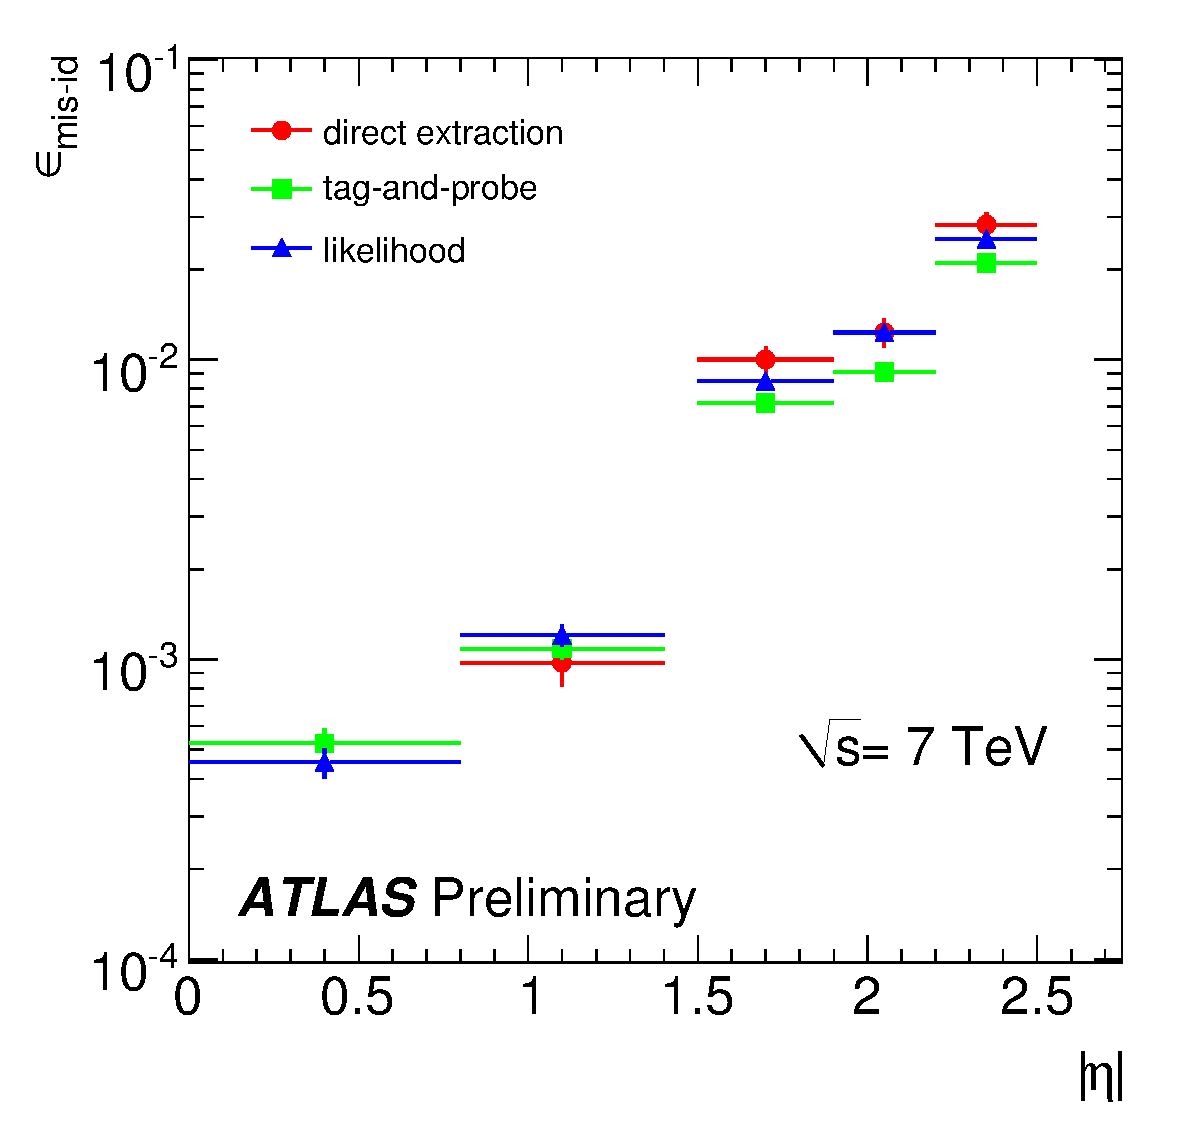
\includegraphics[scale=0.35]{figures/samesign/MisId_data}}
\subfigure[\label{misid:closure}]{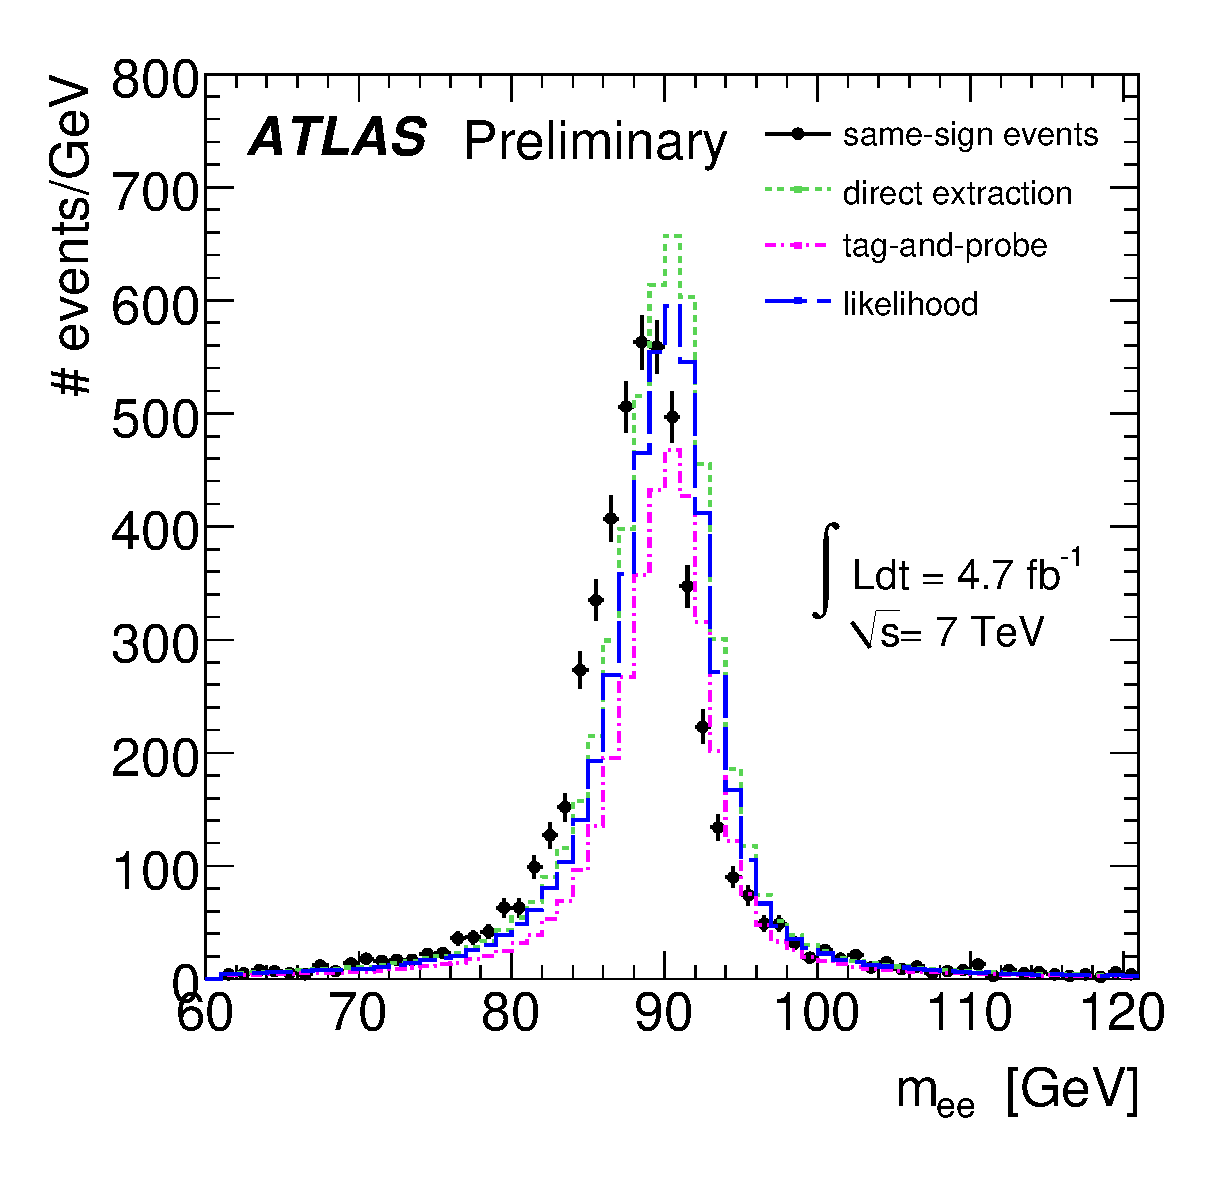
\includegraphics[scale=0.35]{figures/samesign/closure_data}}
\caption{Charge mis-identification rate as a function of the electron $|\eta|$ (a).
    Invariant mass distribution for same-sign and reweighted opposite-sign events around the $Z$-peak (b).}
\end{figure}

%% \section{Background from charge mis-identification}\label{sect:misid}
%% In some events, a pair of opposite-sign leptons are produced and may be reconstructed as a
%% pair of same-sign leptons, if the charge of one of the leptons is mis-identified.

%% This background comes from two main sources: 
%% \begin{itemize}
%% \item
%% incorrect measurement of the sign of the track curvature; this effect is dominant at small curvature corresponding to high transverse momentum.
%% \item 
%% hard bremsstrahlung producing trident electrons 
%% ($e^{\pm} \rightarrow e^{\pm}\gamma^{*} \rightarrow e^{\pm}e^{+}e^{-}$) for which the energy 
%% cluster is assigned to the wrong track, leading to a mis-identification of the charge. This
%% effect represents 90\% of the charge mis-identification contribution.
%% \end{itemize}
%% The rate of charge mis-identification for muons is only affected by
%% the first source, but has been measured to be negligible compared to
%% other backgrounds.

%% \begin{figure}[t]
%% \centering
%% \subfigure[\label{misid:rates}]{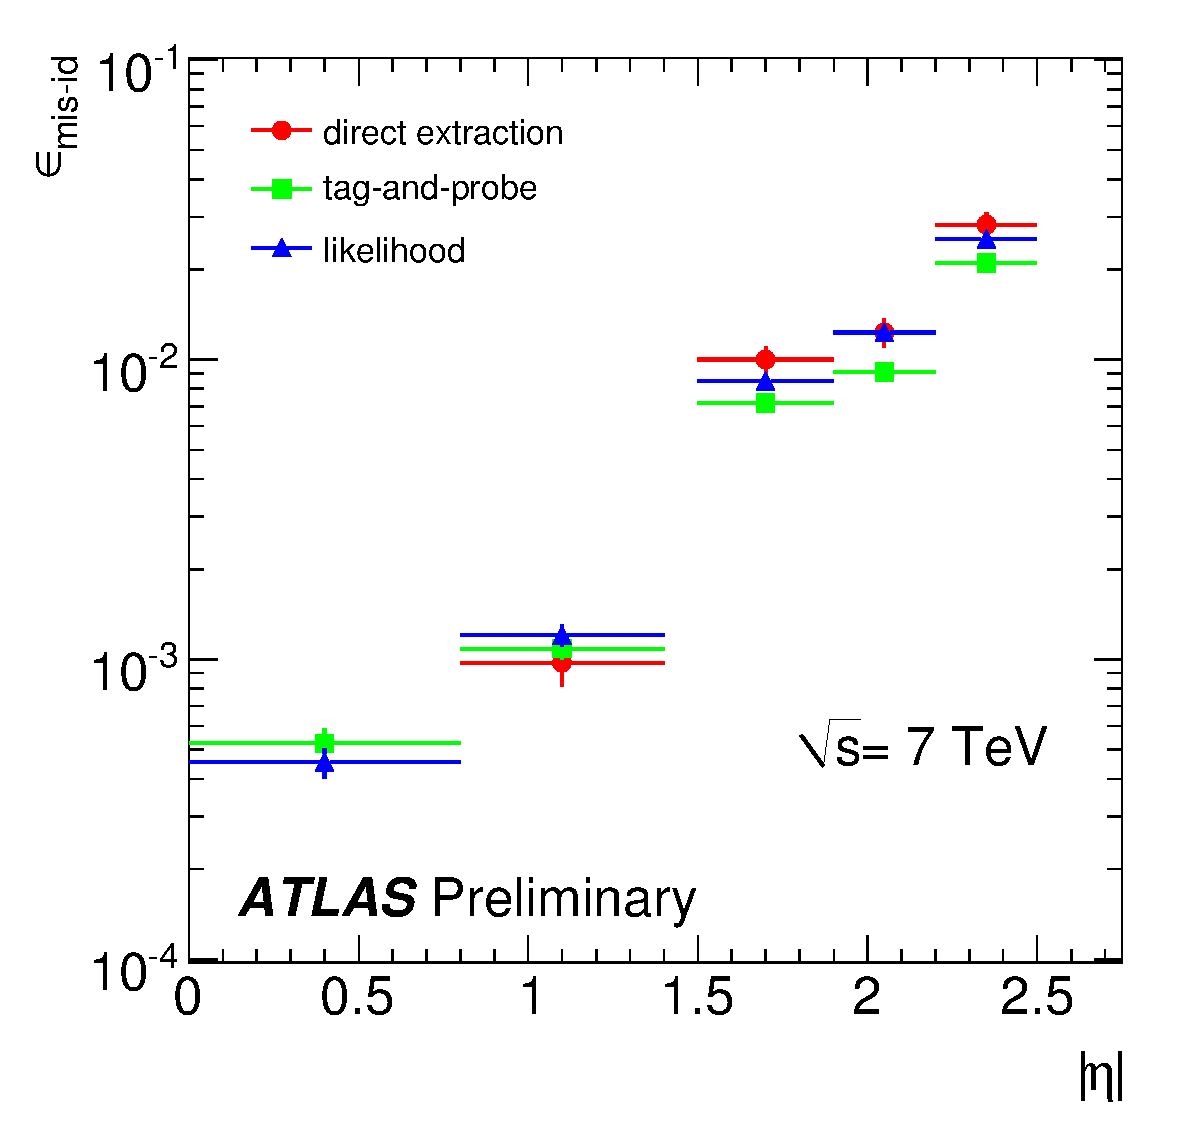
\includegraphics[scale=0.35]{figures/samesign/MisId_data}}
%% \subfigure[\label{misid:closure}]{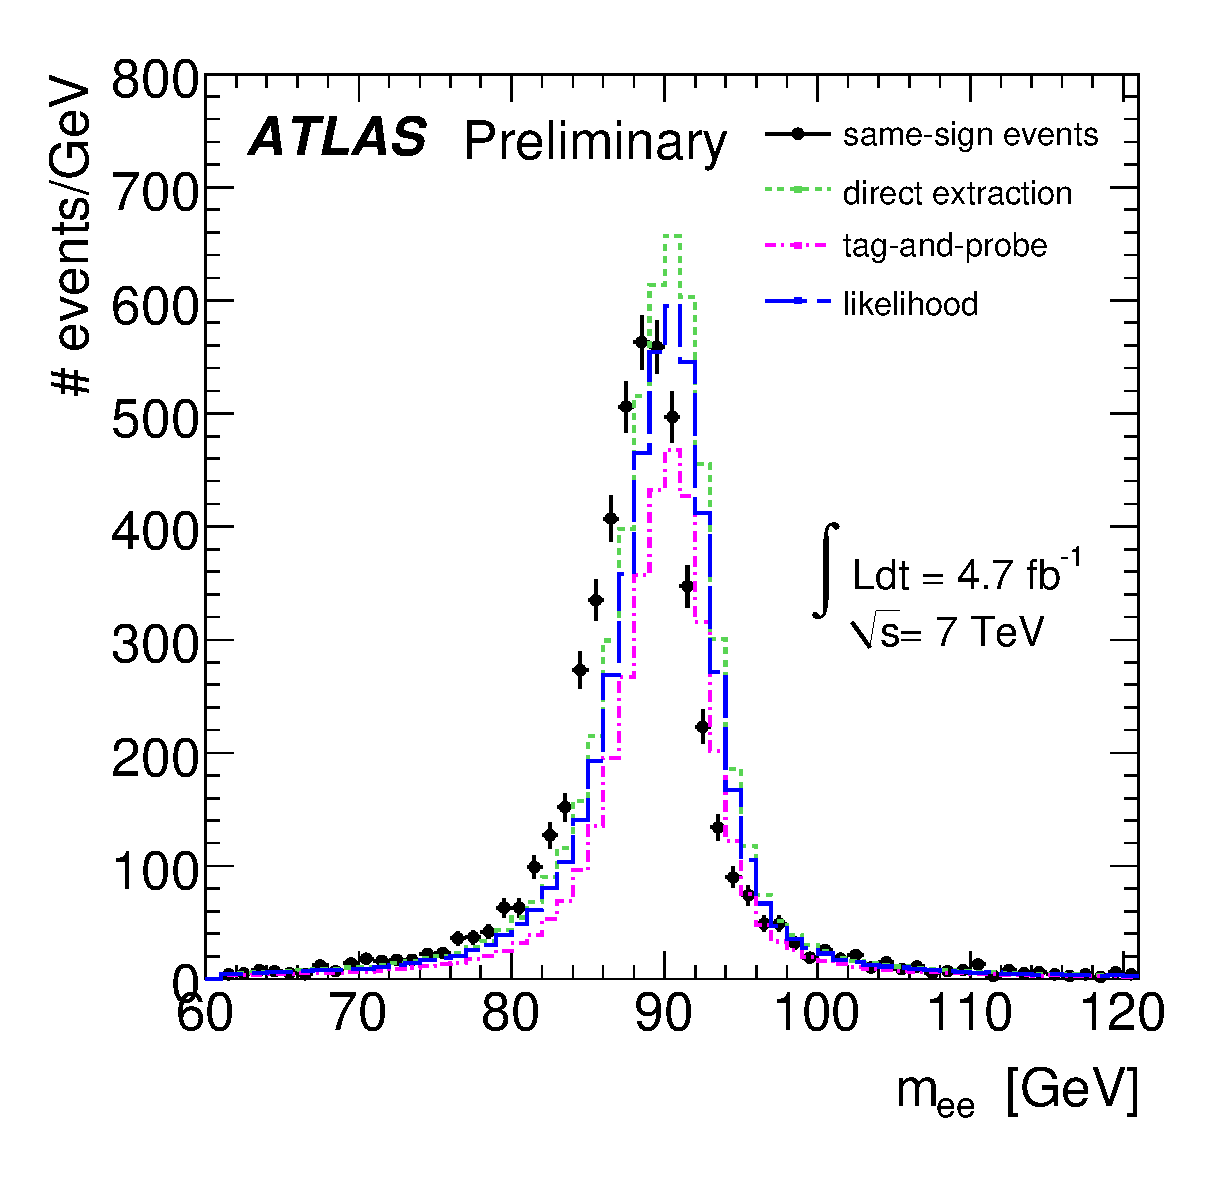
\includegraphics[scale=0.35]{figures/samesign/closure_data}}
%% \caption{Charge mis-identification rate as a function of the electron $|\eta|$ (a).
%%     Invariant mass distribution for same-sign and reweighted opposite-sign events around the $Z$-peak (b).}
%% \end{figure}


The rate of charge mis-identification for electrons is measured by comparing the the rate of same-sign and opposite-sign electron pairs measured in data arising from $Z$ bosons.
Pairs of leptons coming from the decay of $Z$ bosons can be accurately chosen by selecting events with same-flavor leptons whose invariant mass lies beteween 81 \GeV{} and 101 \GeV{}.
Additional backgrounds that may enter this region are subtracted using estimates derived from Monte Carlo.
Using these events, the charge mis-identification rate of electrons was measured as a function of the $p_T$ and $\eta$ of electrons.
These kinematic parameterizations were evaluated by constructing a likelihood functions that describes the two decay products of the $Z$ boson.
The likelihood describes the observed numbers of opposite-sign and same-sign events for each bin in a two-dimensional grid in $|\eta|$ or $p_T$ (for both electrons) as a function of the unknown rates $\epsilon_{\mathrm{mis-id}}(|\eta|)$.
The estimate of the charge mis-identification rate and its uncertainty were evaluated by minimizing this likelihood function when evaluated on measured data.
We found the mis-identification rate of electrons to not depend strongly on the $p_T$ of the electron (given that it is already above the $p_T$ threshold defined by the object selection requirements), and so this dependency is not considered further in the analysis.
The values of $\epsilon_{\mathrm{mis-id}}$ as a function of $|\eta|$ are shown in Figure~\ref{misid:rates}.
To validate this method, two simpler means of paramaterizing the charge mis-identification rate were used, which are referred to as the ``tag-and-probe'' method and the ``direct extraction'' method.
We found good agreement among all three methods. 

%% The rate of charge mis-identification for electrons,
%% $\epsilon_{\mathrm{mis-id}}$, is derived as a function of the electron $|\eta|$
%% from the rate of same-sign and opposite-sign electron pairs in data
%% events from $Z$ bosons with $m_{ee} \in [81, 101] \GeV$. The variation of this rate as a 
%% function of \pT{} is much smaller than the variation with $\eta$, so is neglected in 
%% the parameterization of the the rate. The charge mis-id rate has been
%% calculated with three different methods: tag-and-probe, direct
%% extraction and likelihood. In the tag-and-probe method, the tag
%% electron is required to be within $|\eta| < 0.8$, and the probe electron
%% sign is looked at. In the direct extraction method,
%% both the tag and probe electrons are required to be in the same
%% $|\eta|$ range. Finally, in the likelihood method, all electron pairs
%% are examined: a likelihood function is built as a function of the observed numbers of
%% opposite-sign and same-sign events for each bin in a two-dimensional grid in $|\eta|$ (for both
%% electrons), and of
%% the unknown rates $\epsilon_{\mathrm{mis-id}}(|\eta|)$.
%% The minimization of this likelihood allows the charge mis-identification rate in each
%% $\eta$ bin to be extracted.
%% The values of $\epsilon_{\mathrm{mis-id}}$ as a
%% function of $|\eta|$ are shown in Figure~\ref{misid:rates}.


Having measured the charge mis-identification rate in data, the distribution of background events coming from charge-misidentification was estimated by reweighing opposite-sign events by the probability that exactly one electron in each event has its charge mis-identified.
The accuracy of this estimate was evaluated by comparing the number of same-sign lepton pair events in the $Z$-peak to the number estimated using the above method.
These distributions are presented in Figure~\ref{misid:closure}.
The maximum difference between the estimate as evaluated using the likelihood method and the estimates from the other methods is taken to be a systematic uncertainty on the charge mis-identification background method.

%% used for the systematic uncertainty determination.

%% A closure test is performed by comparing the numbers of events selected in the $Z$-peak 
%% region using same-sign electron pairs (5143 events), and 
%% opposite-sign electron pairs reweighted by the mis-id weight. These distributions are presented
%% in Figure~\ref{misid:closure}. The likelihood method gives the best agreement with the 
%% same-sign rate: 5000 events,
%% while the direct extraction and tag-and-probe methods give higher 
%% and lower rates on average, 5500 and 3700 events respectively.
%% These differences are understood as arising from the different kinematic requirements
%% in the three methods. 
%% Therefore, the nominal estimate is done using the likelihood method, and the two other methods are
%% used for the systematic uncertainty determination. In this closure test,
%% the $Z$-peak for same-sign electrons is shifted to lower values with respect 
%% to opposite-sign electrons because a larger momentum fraction has been radiated for the same-sign case,
%% due to trident electrons.

To estimate the background in the signal region, a selection is defined that is identical to the nominal signal region with the exception that it requires exactly two opposite-sign leptons, as compared to a pair of same-sign leptons with any number of additional leptons.
Events are selected from real data for each of the three signal regions using the above criteria.
These events are then rescaled based on their probability of having the charge of exactly one of the two leptons be mis-identified.

%% The nominal charge mis-identification rate is then applied to data events passing the full signal 
%% selection but requiring an opposite-sign $e^+e^-$ or 
%% $e^{\pm}\mu^{\mp}$ pair, to estimate the charge mis-identification contribution to the same-sign sample.

\section{Backgrounds with leptons originating from jets or photons}\label{sect:fakes}

The largest backgrond for this analysis comes from Standard Model events that include at least one or more ``fake'' leptons in additional to any number of real leptons.
Fake leptons primary come either from the semi-leptonic decay of a $b$ or $c$ hadron which is falsely identified as an isolated lepton originating from the primary vertex or the mis-reconstruction of  $\pi^0$ or photons as leptons.

%% \section{Backgrounds with leptons originating from jets or photons}\label{sect:fakes}
%% The largest SM background source is from events with at least one ``fake'' lepton,
%% in addition to any number of ``real'' leptons that come from the decay of a $W$ or $Z$ boson.
%% The fake leptons may come from the semi-leptonic decay of a $b$ or $c$ hadron,
%% falsely identified as an isolated lepton, or $\pi^0$ or photons mis-reconstructed as leptons.

The nominal object selection uses quality requirements on the track and cluster of selected electrons and muons to reduce the systematic effect of mis-identified leptons.
Cuts on these variables, by design, disproportionatly reject fake leptons relative to real ones.
This fact can be used to directly estimate in data the rate of fake lepton production by reinterpreting the quality criteria as a discriminating variable with discrete values.

To estimate the rate background from fake leptons, we define a looser working point for electron and muon quality in addition to the ``tight'' definition described in the nominal object selection.
Using these definitions, we define probabilities ... BLAH BLAH BLAH

BLAH BLAH BLAH
%% BEGIN BLAH BLAH BLAH HERE

%% To estimate this background, two sets of lepton selection criteria are defined, named 
%% {\it loose} and {\it tight}. The probabilities $r$ and $f$ that a real or fake {\it loose} lepton 
%% passes the {\it tight} criteria are measured using purified control regions and they depend on the
%% characteristics of the event.
%% The matrix method~\cite{Aad:2010ey,Theveneaux-Pelzer:1476909} is then used to estimate the number 
%% of events in the signal region with at least one fake lepton.

%% The {\it tight} lepton definitions are the ones used in the standard selection described in
%% Section~\ref{sect:selection}. 
%% The {\it loose} electron selection is equivalent to the {\it tight} 
%% electron selection with the isolation requirement replaced by a looser cut. The {\it loose} muon selection
%% is equivalent to the {\it tight} muon selection with the isolation requirement removed. We define an
%% {\it anti-tight} lepton as being an exclusively {\it loose} lepton, i.e. required not to be {\it tight}.

%% The number of events that contain
%% two {\it tight} leptons is denoted $N_{TT}$. The number of events with one {\it tight} and one 
%% {\it anti-tight} is denoted $N_{TA}$ or $N_{AT}$, distinguished by $p_T$-ordering.
%% Similarly, the two {\it anti-tight} lepton count is referred to as $N_{AA}$. The total number of
%% events with two {\it loose} leptons is therefore $N^{ll}=N_{TT}+N_{TA}+N_{AT}+N_{AA}$.

%% $N_{RR}^{ll}$ is the number of events that contain two real leptons, the number of events with one 
%% real and one fake leptons is denoted $N_{RF}^{ll}$ or $N_{FR}^{ll}$ depending on the $\pt$ of the 
%% leptons, and the number for two fake leptons is $N_{FF}^{ll}$. The total number of events with
%% two {\it loose} leptons is therefore
%% $N^{ll}=N_{RR}^{ll}+N_{RF}^{ll}+N_{FR}^{ll}+N_{FF}^{ll}$.
%% These numbers are unknown.

%% The number of events with two {\it tight} leptons, our signal region sample, can be written as
%% $N_{TT}=N_{RR}^{tt}+N_{RF}^{tt}+N_{FR}^{tt}+N_{FF}^{tt}$ and the final fake estimation is
%% $N_{TT}^{\mathrm{fakes}}=r_1 f_2 N_{RF}^{ll}+f_1 r_2 N_{FR}^{ll}+f_1 f_2 N_{FF}^{ll}$, where $r_1$ and $f_1$
%% are the probabilities for the first lepton, and $r_2$ and $f_2$ for the second lepton.

%% Linear expressions are obtained for the observed yields $N_{TT,TA,AT,AA}$ as a function 
%% of the unknown numbers $N_{RR,RF,FR,FF}^{ll}$ and the measured rates $r$ and $f$. 
%% These linear expressions form a 
%% matrix that is inverted to extract the real and fake content of the selected dilepton event sample:
%% \begin{equation}
%%   \begin{bmatrix} N_{TT} \\ N_{TA} \\ N_{AT} \\ N_{AA} \\ \end{bmatrix} =
%%   \begin{bmatrix}  r_1 r_2        & r_1 f_2       & f_1 r_2        & f_1 f_2         \\
%%     r_1 (1-r_2)     & r_1 (1-f_2)     & f_1 (1-r_2)     & f_1 (1-f_2)     \\
%%     (1-r_1)r_2    & (1-r_1)f_2     & (1-f_1)r_2     & (1-f_1)f_2     \\
%%     (1-r_1)(1-r_2) & (1-r_1)(1-f_2) & (1-f_1)(1-r_2) & (1-f_1)(1-f_2) \\             
%%   \end{bmatrix}
%%   \begin{bmatrix} N_{RR}^{ll} \\ N_{RF}^{ll} \\ N_{FR}^{ll} \\ N_{FF}^{ll} \\ \end{bmatrix}
%%   \label{matrice}
%% \end{equation}

%% The value of $r$ was determined with a tag-and-probe method on 
%% $Z \rightarrow e^+e^-/\mu^+\mu^-$ events where the overlap removal between leptons and jets (see 
%% Section~\ref{sect:selection}) is applied with {\it loose} leptons.

%% The value of $f$ for fake electrons is estimated in a sample with at least one jet and exactly one 
%% {\it loose} electron, 
%% with a cut on the distance between the leading jet and the lepton, with the overlap 
%% removal performed with {\it loose} electrons, and with $\met{}<20 \GeV$ in order to 
%% enrich the sample in multijets.

%% The value of $f$ for fake muons was determined from data for events with one {\it loose} muon and
%% in a low transverse $W$ mass region, with an 
%% inverted triangular cut: $m_T(W)<20 \GeV$ and $\met{}+m_T(W)<60 \GeV$. 

%% To measure the yield of events with at least one fake lepton, 
%% we use the same cuts as the full analysis but ask for 
%% {\it loose} leptons instead of {\it tight} leptons. These events are weighted with a weight that depends
%% on some kinematic variables: the weights for electrons 
%% are parametrized versus $|\eta|$ and \pt{}, while for muons they are parametrized in muon 
%% $|\eta|$ and \pt{} of the leading jet in order to account for dependencies on muon detector acceptance and 
%% hadronic activity from hard jets affecting the muon isolation.

%% Trident electrons have a smaller probability to pass the {\it tight} selection than normal electrons, 
%% thus a fraction of trident electrons will be included in the fake lepton estimate from the matrix method.
%% We therefore estimate and remove this double-counting by applying the matrix method to the same-sign
%% events with a dilepton mass inside
%% the $Z$-peak, dominated by trident electrons. This estimate results in 22\% of mis-id events that
%% are captured as fake background: we scale the estimated charge mis-identification 
%% contribution down by 78\% to remove the overlap between the two estimates.

BLAH BLAH BLAH
%% END BLAH BLAH BLAH HERE

\section{Background control regions}

The analysis described in this section uses a number of sophisticaed techniques to estimate the size of backgrounds.
The accuracy of these techniques were evaluated using a number of control regions, each designed to enchance a particular background process and to allow for comparison of background estimates to data.
These regions are defined to be orthognal to the nominal signal regions and are designed to have minimial signal contamination.

%% \section{Background control regions}
%% To validate the modeling of the SM backgrounds, several control regions are
%% examined. Control regions are orthogonal to the signal region and defined by selections that
%% suppress possible signal contributions.

The primary control region considered partially inverts the cut on \HT{} by requiring $100 GeV < \HT{} < 500 GeV$ and eliminates the cut on \met{} to increase the number of background events.
The expected and observed number of events observed in this control region are in good agreement.

A second control region which maintains a cut requiring high \HT{} is also defined.
This region requires at least one $b$-jet (with no other requirement on the number of jets), $\HT>400 \GeV$ but imposes $\met<40 \GeV$ in order to be orthogonal to the signal region. 
The resulting number of events can be seen in Table~\ref{ctrl:met_yield} and shows good agreement within the very low statistics.


\begin{table}[p]
  \begin{center}
    \caption{Observed number of events in the main control regions and the expected number of background events in those regions, including statistical (first) and systematic (second) uncertainties.
        For the Monte Carlo samples, systematic uncertainties shown here include only uncertainties on the overall production cross-section
        The expected signal contamination from two example models is also shown, with statistical uncertainties only. 
        The last two rows show the number of expected and observed events when applying an additional cut on \met{}.}\label{ctrl:ht2j_yield}
    \begin{tabular}{l|c|c|c}
      \hline\hline
       & \multicolumn{3}{c}{Channel} \\
      \cline{2-4}
      Backgrounds & $ee$ & $e\mu$ & $\mu\mu$ \\
      \hline
      Mis-id & $5.2\pm 0.3 \pm 0.6$ & $7.9\pm 0.3 \pm 1.0$ & --- \\
      Fakes & $10.0\pm 5.3 \pm 5.0$ & $34\pm 5 \pm 14$ & $17.4\pm 1.8 \pm 5.2$ \\
      \hline
      Diboson & & & \\
      $\bullet$ $WZ/ZZ$+jets & $0.69\pm 0.23 \pm 0.12$ & $2.15\pm 0.36\pm 0.37$ & $2.17\pm 0.40\pm 0.44$ \\
      $\bullet$ $W^{\pm}W^\pm$+2 jets & $0.06\pm 0.03\pm 0.03$ & $0.27\pm 0.06\pm 0.14$ & $0.15\pm 0.04\pm 0.07$ \\
      \hline
      $t\bar{t}+W/Z$ & & & \\
      $\bullet$ $t\bar{t}W$(+jet) & $0.77\pm 0.04\pm 0.17$ & $3.34\pm 0.09\pm 0.73$ & $2.06\pm 0.07\pm 0.45$ \\
      $\bullet$ $t\bar{t}Z$(+jet) & $0.32\pm 0.02\pm 0.12$ & $1.33\pm 0.05\pm 0.48$ & $0.88\pm 0.04\pm 0.32$ \\
      $\bullet$ $t\bar{t}W^{\pm}W^\mp$ & $0.008\pm 0.001\pm 0.002$ & $0.033\pm 0.001\pm 0.010$ & $0.024\pm 0.001\pm 0.007$ \\
      \hline
      Total & $17.0 \pm 5.3 \pm 5.0$ & $49 \pm 5 \pm 14$ & $22.7 \pm 1.8 \pm 5.2$ \\
      \hline
      Observed & 16 & 34 & 18 \\
      \hline
      Signal contamination & & & \\
      $\bullet$ b$^\prime$ / $T_{5/3}$ (550~\GeV{}) & $0.26\pm0.04$ & $0.96\pm0.08$ & $0.76\pm0.07$ \\
      $\bullet$ 4 tops ($\sigma=12.6$~fb) & $0.012\pm0.003$ & $0.046\pm0.005$ & $0.027\pm0.004$ \\
      \hline
      \multicolumn{4}{c}{Including $\met{}>40 \GeV$} \\
      \hline
      Total & $11.3 \pm 4.0 \pm 3.6$ & $36 \pm 5 \pm 10$ & $16.1 \pm 1.4 \pm 3.6$ \\
      \hline
      Observed & 9 & 23 & 13 \\
      \hline
    \end{tabular}

    \vspace{1cm}

    \caption{Observed number of events in the data and expected number of background events with 
        statistical (first) and systematic (second) uncertainties for the second control region
        selection. For the Monte Carlo samples, systematic uncertainties include only the production 
        cross section uncertainties.}\label{ctrl:met_yield}
    \begin{tabular}{l|c|c|c}
      \hline\hline
       & \multicolumn{3}{c}{Channel} \\
      \cline{2-4}
      Backgrounds & ee & e$\mu$ & $\mu\mu$ \\
      \hline
      Mis-id & $0.33\pm 0.08 \pm 0.04$ & $0.17\pm 0.04 \pm 0.02$ & --- \\
      Fakes & $2.3\pm 3.2 \pm 1.1$ & $1.2\pm 1.2 \pm 0.5$ & $0.71\pm 0.32\pm 0.21$ \\
      \hline
      Diboson & & & \\
      $\bullet$ $WZ/ZZ$+jets & $0.20\pm 0.21 \pm 0.05$ & $0.92\pm 0.33\pm 0.15$ & $0.25\pm 0.19\pm 0.06$ \\
      $\bullet$ $W^{\pm}W^\pm$+2 jets & $0\pm 0.01$ & $0.014\pm 0.014\pm 0.007$ & $0.03\pm 0.02\pm 0.01$ \\
      \hline
      $t\bar{t}+W/Z$ & & & \\
      $\bullet$ $t\bar{t}W$(+jet) & $0.10\pm 0.02\pm 0.02$ & $0.31\pm 0.03\pm 0.07$ & $0.18\pm 0.02\pm 0.04$ \\
      $\bullet$ $t\bar{t}Z$(+jet) & $0.10\pm 0.01\pm 0.03$ & $0.33\pm 0.02\pm 0.12$ & $0.22\pm 0.02\pm 0.08$ \\
      $\bullet$ $t\bar{t}W^{\pm}W^\mp$ & $0.0022\pm 0.0004\pm 0.0007$ & $0.0064\pm 0.0007\pm 0.0019$ & $0.0046\pm 0.0005\pm 0.0014$ \\
      \hline
      Total & $3.0 \pm 3.2 \pm 1.1$ & $2.9 \pm 1.2 \pm 0.5$ & $1.4 \pm 0.4 \pm 0.2$ \\
      \hline
      Observed & 1 & 4 & 0 \\
      \hline
    \end{tabular}
  \end{center}
\end{table}



%% The main control region inverts the \HT{} selection by requiring $\HT{} \in [100,500] \GeV$ and
%% does not include the cut on \met{}, in order to increase the number of events. 

%% \begin{table}[p]
%%   \begin{center}
%%     \caption{Observed number of events in the data and expected number of background events with 
%%         statistical (first) and systematic (second) uncertainties for the main control region
%%         selection. For the Monte Carlo samples, systematic uncertainties include only the production 
%%         cross section uncertainties.
%%         Examples of expected contamination from two signals are also shown, with
%%         statistical uncertainties only. The last two rows show the number of expected and observed
%% 	events when applying the cut on \met{}.}\label{ctrl:ht2j_yield}
%%     \begin{tabular}{l|c|c|c}
%%       \hline\hline
%%        & \multicolumn{3}{c}{Channel} \\
%%       \cline{2-4}
%%       Backgrounds & $ee$ & $e\mu$ & $\mu\mu$ \\
%%       \hline
%%       Mis-id & $5.2\pm 0.3 \pm 0.6$ & $7.9\pm 0.3 \pm 1.0$ & --- \\
%%       Fakes & $10.0\pm 5.3 \pm 5.0$ & $34\pm 5 \pm 14$ & $17.4\pm 1.8 \pm 5.2$ \\
%%       \hline
%%       Diboson & & & \\
%%       $\bullet$ $WZ/ZZ$+jets & $0.69\pm 0.23 \pm 0.12$ & $2.15\pm 0.36\pm 0.37$ & $2.17\pm 0.40\pm 0.44$ \\
%%       $\bullet$ $W^{\pm}W^\pm$+2 jets & $0.06\pm 0.03\pm 0.03$ & $0.27\pm 0.06\pm 0.14$ & $0.15\pm 0.04\pm 0.07$ \\
%%       \hline
%%       $t\bar{t}+W/Z$ & & & \\
%%       $\bullet$ $t\bar{t}W$(+jet) & $0.77\pm 0.04\pm 0.17$ & $3.34\pm 0.09\pm 0.73$ & $2.06\pm 0.07\pm 0.45$ \\
%%       $\bullet$ $t\bar{t}Z$(+jet) & $0.32\pm 0.02\pm 0.12$ & $1.33\pm 0.05\pm 0.48$ & $0.88\pm 0.04\pm 0.32$ \\
%%       $\bullet$ $t\bar{t}W^{\pm}W^\mp$ & $0.008\pm 0.001\pm 0.002$ & $0.033\pm 0.001\pm 0.010$ & $0.024\pm 0.001\pm 0.007$ \\
%%       \hline
%%       Total & $17.0 \pm 5.3 \pm 5.0$ & $49 \pm 5 \pm 14$ & $22.7 \pm 1.8 \pm 5.2$ \\
%%       \hline
%%       Observed & 16 & 34 & 18 \\
%%       \hline
%%       Signal contamination & & & \\
%%       $\bullet$ b$^\prime$ / $T_{5/3}$ (550~\GeV{}) & $0.26\pm0.04$ & $0.96\pm0.08$ & $0.76\pm0.07$ \\
%%       $\bullet$ 4 tops ($\sigma=12.6$~fb) & $0.012\pm0.003$ & $0.046\pm0.005$ & $0.027\pm0.004$ \\
%%       \hline
%%       \multicolumn{4}{c}{Including $\met{}>40 \GeV$} \\
%%       \hline
%%       Total & $11.3 \pm 4.0 \pm 3.6$ & $36 \pm 5 \pm 10$ & $16.1 \pm 1.4 \pm 3.6$ \\
%%       \hline
%%       Observed & 9 & 23 & 13 \\
%%       \hline
%%     \end{tabular}

%%     \vspace{1cm}

%%     \caption{Observed number of events in the data and expected number of background events with 
%%         statistical (first) and systematic (second) uncertainties for the second control region
%%         selection. For the Monte Carlo samples, systematic uncertainties include only the production 
%%         cross section uncertainties.}\label{ctrl:met_yield}
%%     \begin{tabular}{l|c|c|c}
%%       \hline\hline
%%        & \multicolumn{3}{c}{Channel} \\
%%       \cline{2-4}
%%       Backgrounds & ee & e$\mu$ & $\mu\mu$ \\
%%       \hline
%%       Mis-id & $0.33\pm 0.08 \pm 0.04$ & $0.17\pm 0.04 \pm 0.02$ & --- \\
%%       Fakes & $2.3\pm 3.2 \pm 1.1$ & $1.2\pm 1.2 \pm 0.5$ & $0.71\pm 0.32\pm 0.21$ \\
%%       \hline
%%       Diboson & & & \\
%%       $\bullet$ $WZ/ZZ$+jets & $0.20\pm 0.21 \pm 0.05$ & $0.92\pm 0.33\pm 0.15$ & $0.25\pm 0.19\pm 0.06$ \\
%%       $\bullet$ $W^{\pm}W^\pm$+2 jets & $0\pm 0.01$ & $0.014\pm 0.014\pm 0.007$ & $0.03\pm 0.02\pm 0.01$ \\
%%       \hline
%%       $t\bar{t}+W/Z$ & & & \\
%%       $\bullet$ $t\bar{t}W$(+jet) & $0.10\pm 0.02\pm 0.02$ & $0.31\pm 0.03\pm 0.07$ & $0.18\pm 0.02\pm 0.04$ \\
%%       $\bullet$ $t\bar{t}Z$(+jet) & $0.10\pm 0.01\pm 0.03$ & $0.33\pm 0.02\pm 0.12$ & $0.22\pm 0.02\pm 0.08$ \\
%%       $\bullet$ $t\bar{t}W^{\pm}W^\mp$ & $0.0022\pm 0.0004\pm 0.0007$ & $0.0064\pm 0.0007\pm 0.0019$ & $0.0046\pm 0.0005\pm 0.0014$ \\
%%       \hline
%%       Total & $3.0 \pm 3.2 \pm 1.1$ & $2.9 \pm 1.2 \pm 0.5$ & $1.4 \pm 0.4 \pm 0.2$ \\
%%       \hline
%%       Observed & 1 & 4 & 0 \\
%%       \hline
%%     \end{tabular}
%%   \end{center}
%% \end{table}

%% For the main control region, 
%% the predicted number of background events, including only the dominant systematic
%% uncertainties --- production cross sections for the Monte Carlo samples and global systematic
%% uncertainties on the data-driven backgrounds as explained in Section~\ref{sect:syst} --- are
%% shown in Table~\ref{ctrl:ht2j_yield}, as well as the observed number of events in the data.
%% Expected and observed numbers agree within uncertainties. The expected numbers of events from
%% two examples of signals are also shown in Table~\ref{ctrl:ht2j_yield} and are found to be
%% negligible in this control region.


%% As the main control region concentrates on the low
%% \HT{} region, a second control region, with high \HT{}, is defined.
%% The second control region requires at least one $b$-jet 
%% (and no other requirement on the number of jets), 
%% $\HT>400 \GeV$ and $\met<40 \GeV$ in order to be
%% orthogonal to our signal region. The resulting number of events can be seen in Table~\ref{ctrl:met_yield}
%% and shows good agreement within the very low statistics.

\section{Systematic uncertainties}\label{sect:syst}
Several sources of systematic uncertainty have been considered for both signal and background estimates,
including background that have been estimated using both Monte Carlo and data-driven techniques.
Systematic uncertainties that come from Monte Carlo simulations can be evaluated by modifying parameters of the simulation,
rerunning the simulation and re-applying the signal selection, and observing the difference in the expected rate of signal or background.
Since this process is computationally intensive, for the majority of systematic uncertainties,
one does not actually modify parameters at the generator level and generate new simulated events.
Instead, it is faster to apply weights or to modify the kinematics of already-generated events
such that the overall distribution approximates the  expected distribution under a systematic change
in an underlying parameter.
Systematic uncertainties on backgrounds estimated using data-driven technqiues tend to be more complicated to evaluate
as one does not have a direct handle on the underlying variables that paramaterize systematic uncertainties.
Instead, one must rely on techniques for evaluating those uncertainties that are specific to the background estimate being used, 
and often very conservative estimates are used to avoid under-estimation of these errors.


\subsubsection{Luminosity and production cross-sections}
Uncertainty on the measured value of integrated luminosity leads to an uncertainty on the overall scale of backgrounds that are derived using Monte-Carlo.
The uncertainty on the luminosity has been estimated from van der Meer scans and is 3.9\%~\cite{Aad:2011dr,ATLAS-CONF-2011-116}. 

%These uncertainties affect the overall scale of the various samples.
%The uncertainty on the measured luminosity from van der Meer scans was estimated to be 3.7\%. %~\cite{lumi}. 

% Not sure what the most up-to-date reference is for this...
% ATLAS Collaboration, ATLAS-CONF-2011-116, http://cdsweb.cern.ch/record/1376384.
% ATLAS Collaboration, Eur. Phys. J. C71, 1630 (2011).
In addition, uncertainties on the overall cross-sections of Monte-Carlo samples are considered,
and these are determined using dedicated studies of Monte-Carlo generators.
Uncertainties on Monte Carlo cross sections are included separately for each background processes considered.
The uncertainty on $t \overline{t}$ processes with an additional boson are taken to be 30\% for a W boson 
and 50\% for a Z boson\footnote{\url{https://twiki.cern.ch/twiki/bin/viewauth/AtlasProtected/TTplusV}}.
% Cite these references
% Page: https://twiki.cern.ch/twiki/bin/viewauth/AtlasProtected/TTplusV
% Reference: http://arxiv.org/pdf/1204.5678v1.pdf
The uncertainty on the cross-section of $WZ$ and $ZZ$ events is taken to be 5\% with an additional contribution of 24\% per jet added in quadrature included, making the total cross-section uncertainty 34\%.
% From Here: https://twiki.cern.ch/twiki/bin/viewauth/AtlasProtected/TopSystematicUncertainties2011#Systematics_Affecting_Other_MC
% Reference: arXiv:1012.1792
For the $W^{\pm}W^{\pm}$+2 jets sample, the uncertainty on the cross-section is 50\%.
The uncertainty on the $t\bar{t}W^{\pm}W^{\mp}$ has been evaluated by setting the renormalization
and factorization scales to the values of 0.5 and 2, and rerunning the Madgraph event generator 
in these two configurations. 
The difference with respect to the standard configuration has been used to set the up
(+35\%) and down (-24\%) cross-section uncertainties.

ELIMINATE THIS IF THE SAME AS ABOVE:
Uncertainties on Monte Carlo background cross sections depend on the process: 
30\% for the $t\bar{t}W$(+jet) sample, 
34\% for the $WZ$ and $ZZ$ samples, 
$+35$\% and $-24$\% for the $t\bar{t}W^{\pm}W^{\mp}$ sample, 
and 50\% for the $W^{\pm}W^{\pm}$+2 jets and $t\bar{t}Z$(+jet) samples. 


%% I'm assuming I wrote much of these below
\subsubsection{Uncertainties on object kinematics from Monte Carlo}
Uncertainties on the trigger, jet and lepton efficiencies, energy or momentum calibration,
and trigger and object resolution lead to systematic uncertainties on the signal and background acceptance.
% Their effect is evaluated by varying each parameter independently within its uncertainty and recomputing the yield of each sample.
The modeling of lepton triggers as well as reconstruction and identification efficiencies in
Monte Carlo simulation are corrected by scale factors, which are a function of lepton kinematics.
These scale factors, as well as their uncertainties, are obtained from studies of $Z \rightarrow \mu \mu$ and $Z \rightarrow e e$ decays.
The uncertainty on the overall yield due uncertainties on trigger, reconstruction, and identification efficiencies
are obtained by independently shifting these scale factors up and down by one standard deviation.

% jet %~\cite{atlasjets}
Uncertainties on the efficiency, energy or momentum calibration, and resolution of leptons and jets
lead to systematic uncertainties on the signal and background acceptances and distributions of discriminating variables.
These uncertainties are summarised in Tables~\ref{tab:systematicsBprime}, \ref{tab:systematicsT53} and
\ref{tab:systematics4t} for signals and in Table~\ref{tab:systematicsBG} for the background samples.
They are evaluated by shifting the energy or momenta of objects by one standard deviation in each direction,
where the size of each standard deviation associated with each uncertainty is determined by detailed studies.
Shifts for each systematic are applied separately.

%These shifts are propagated to templates of discriminating variables,
%meaning that the effect of calibration and resolution systematic uncertainties are considered for each bin.
When measuring the effect of systematic uncertaities, changes in the momenta of reconstructed objects are applied to the calculation of \met{}.
In addition, uncertainties specific to the calculation of \met{} are considered.
The effect of Pile-Up on the \met{} resolution is taken to be 6.6\%,
and uncertainties on $\met{}$ also include contributions arising from calorimeter cells not associated with jets and from soft jets with 7 $\GeV\ < \pt  < 20 \GeV{}$.
The latter two uncertainties are not considered to be independent, but rather are applied coherently.

The detailed results of the size of systematic uncertainties for the various signals and backgrounds
considered in this analysis are describe in Appendix~\ref{App:SameSignSystematics}.

%% Reduce the following by a lot...
\subsubsection{PDF uncertainty}
Uncertainties on the parton distribution functions used to generate signal events lead to uncertainties on the measured cross-section.
The parton distribution function used in this analysis were not calculated from first principles but are determined experimentally.
As such, there are a variety of uncertainties that that come from the models used to extract the PDF's
and the parameters of the PDF's themselves.
The uncertainty due to the modeling of the parton distribution function is evaluated by applying weights to reconstructed events
that are designed to mimic the effect of changing the many underlying parameters of the parton distribution functions.
The maximum and minimum shifts in the signal acceptance due to changes in the PDF using this reweighting method
are found to be $+1.4$\% and $-1.1$\%, with an average shift across channels and signal samples of 0.6\%.

%% In this setup MRST LO** PDF (LHAPDF set number 20651)~\cite{LOstar,LOstarstar} is the default PDF %(ATL-PHYS-PUB-2011-009)
%% and the "ATLAS Underlying Event Tune 2B" (AUET2B) tune~\cite{AUET2B} is the corresponding UE tune.
%% MRST LO** is an LO generator, thus the following alternative LO PDFs have been used in this study:
%% \begin{itemize}
%% %
%% \item CTEQ6L1 (10042) - with LO fit and LO $\alpha_S$~\cite{CTEQ6};
%% %
%% \item MSTW2008LO (21000)~\cite{MSTW2008LO};
%% %
%% \item MRST LO* (20650)~\cite{MRSTLOX};
%% %
%% \item CT09MC2 (10772)~\cite{CT09MC2};
%% %
%% \end{itemize}

\subsubsection{Initial and final state radiation}
Changes in the amount of initial and final state radiation in simulated events will
effect the rate of signal entering the acceptance region, as additional gluon
emmisions from inital or final state legs of Feynman diagrams will produce
additional jets.
To evaluate the size of this effect, dedicated simulation samples with varying levels of
ISR and FSR were produced by changing the parton shower (PS) parameters in Pythia, 
as described in table~\ref{tab:ISFFRS}.
\begin{table}[htbp]
\begin{center}
\caption{\textit{Pythia parameters changed to produce samples with more and less parton shower. Those samples were used to estimate ISR, FSR systematic uncertainty.}}
\label{tab:ISFFRS}
\begin{tabular}{c|c|c|l}
\hline\hline
Pythia parameter & Less PS & More PS & Comment\\
PARP(67) & 0.70   & 1.75   & controls high-pt ISR branchings phase-space \\
PARP(64) & 3.60   & 0.60   & multiplicative factor of the momentum scale squared\\
         &        &        & in running $\alpha_s$, used in ISR \\
PARP(72) & 0.2150 & 0.6450 & multiplicative factor of the $\Lambda_{QCD}$\\
         &        &        & in running $\alpha_s$, used in FSR \\
PARJ(82) & 1.66   & 0.5    & FSR low-pt cutoff \\
\hline
\end{tabular}
\end{center}
\end{table}
About 150k events were produced for each signal dataset, and the full reconstruction and signal selection was run on these events.
The change in yield due to changes in ISR/FSR is evaluated of the order of 6\%.



\subsubsection{Uncertainties affecting the data-driven backgrounds}
The uncertainty on the overall scale of the charge mis-identification background in the signal region is derived from a comparison of the charge-flip rate extracted by several methods.
The primary technique, which uses the likelihood method, is compared to the alternative Tag-and-Probe and Direct Extraction methods (see section~\ref{chap:smbkg}).
Based on these methods, an overall uncertainty of 12\% is attributed to the Charge-Flip background.
Based on this comparison, an overall uncertainty of 12\% is attributed to the mis-id background.

Uncertainties on the estimates of background coming from fake leptons are estimated by modifying the efficiency and fake rate estimates that
are used by the Matrix Method.
To estimate the uncertainty on backgrounds that include fake electrons, a separate {\it loose} electron definition was considered and the Matrix Method was recalculated.
For the uncertainty due to fake muons, the a separate definition of the multijet enriched region was consider, and, in addition, the efficiencies and fake rates were paramaterized in terms of the number of jets instead of the leading jet \pT{}.
Uncertainties on the estimate of background coming from fake leptons are 50\% for the $ee$ channel, 40\% for the $e\mu$ channel, and 30\% for the $\mu\mu$ channel.


%% \section{Systematic uncertainties}\label{sect:syst}
%% Several systematic uncertainties have been considered, and their estimates are summarized below.

%% \section{Uncertainties affecting the Monte Carlo samples}
%% Uncertainties in the jet and lepton efficiency,
%% energy or momentum calibration, and resolution lead to systematic uncertainties on the signal
%% and background acceptance. Their effect is evaluated by varying each parameter independently
%% within its uncertainty and recomputing the yield of each sample.

%% The uncertainty on the luminosity has been estimated from van der Meer 
%% scans and is 3.9\%~\cite{Aad:2011dr,ATLAS-CONF-2011-116}. 
%% Uncertainties on Monte Carlo background cross sections depend on the process:
%% 30\% for the $t\bar{t}W$(+jet) sample, 34\% for the $WZ$ and $ZZ$ samples,
%% $+35$\% and $-24$\% for the $t\bar{t}W^{\pm}W^{\mp}$ sample, and
%% 50\% for the $W^{\pm}W^{\pm}$+2 jets
%% and $t\bar{t}Z$(+jet) samples. They are the largest systematic uncertainties for the
%% backgrounds estimated from simulation.

%% \section{Uncertainties affecting the data-driven backgrounds}

%% The uncertainty on the overall scale of the charge mis-identification background in the signal region 
%% is derived  from a comparison of the mis-id rate extracted by the three different methods already
%% discussed. Based on this comparison, an overall uncertainty of 12\% is attributed to the mis-id background.

%% Uncertainties on the estimate of background coming from fake leptons are 50\% for the $ee$ 
%% channel, 40\% for the $e\mu$ channel, and 30\% for the $\mu\mu$ channel.
%% For the electron case, the uncertainty was estimated by using different {\it loose} electron 
%% definitions. For the muon case, it was estimated by changing the definition of the multijet 
%% enriched region, and using the number of jets, instead of the leading jet \pT{}, for the
%% weight parametrization.


\section{Results}\label{sect:results}
After applying the selection to the data, we find four events in the signal region, with $5.6\pm1.7$ expected background events. 
The details of the observed number of events are shown in Table~\ref{finalyield}, as well as the total expected number of background events. 
No significant excess is observed in the data, therefore limits on the signals are computed in the following section.

The distributions of the \met{} and \HT{} variables observed in data are compared to the background estimates in Figure~\ref{fig:signal} and show a good agreement.

\begin{table}[t]
  \begin{center}
    \caption{Observed number of events in data and expected number of background events, including statistical (first) and systematic (second) uncertainties, in signal region selection.}\label{finalyield}
    \begin{tabular}{l|c|c|c}
      \hline\hline
       & \multicolumn{3}{c}{Channel} \\
      \cline{2-4}
      Backgrounds & $ee$ & $e\mu$ & $\mu\mu$ \\
      \hline
      Mis-id & $0.13\pm 0.04 \pm 0.02$ & $0.23\pm 0.04 \pm 0.03$ & --- \\
      Fakes & $0.5\pm 1.1 \pm 0.3$ & $0.8\pm 1.1 \pm 0.3$ & $0.13\pm 0.13\pm 0.04$ \\
      \hline
      Diboson & & & \\
      $\bullet$ $WZ/ZZ$+jets & $0.19\pm 0.20 \pm 0.07$ & $0.34\pm 0.21\pm 0.13$ & $0.28\pm 0.22\pm 0.10$ \\
      $\bullet$ $W^{\pm}W^\pm$+2 jets & $0.06\pm 0.03\pm 0.03$ & $0.07\pm 0.03\pm 0.03$ & $0.03\pm 0.02\pm 0.03$ \\
      \hline
      $t\bar{t}+W/Z$ & & & \\
      $\bullet$ $t\bar{t}W$(+jet) & $0.23\pm 0.02\pm 0.07$ & $0.79\pm 0.04\pm 0.24$ & $0.57\pm 0.04\pm 0.18$ \\
      $\bullet$ $t\bar{t}Z$(+jet) & $0.17\pm 0.02\pm 0.09$ & $0.61\pm 0.03\pm 0.31$ & $0.33\pm 0.02\pm 0.17$ \\
      $\bullet$ $t\bar{t}W^{\pm}W^\mp$ & $0.008\pm 0.001\pm 0.002$ & $0.023\pm 0.001\pm 0.007$ & $0.016\pm 0.001\pm 0.005$ \\
      \hline
      Total & $1.3 \pm 1.1 \pm 0.3$ & $2.9 \pm 1.1 \pm 0.5$ & $1.36 \pm 0.26 \pm 0.27$ \\
      \hline
      Observed & 2 & 2 & 0 \\
      \hline
    \end{tabular}
  \end{center}
\end{table}

\begin{figure}[t]
\centering
\subfigure[\label{sig_met_ee}]{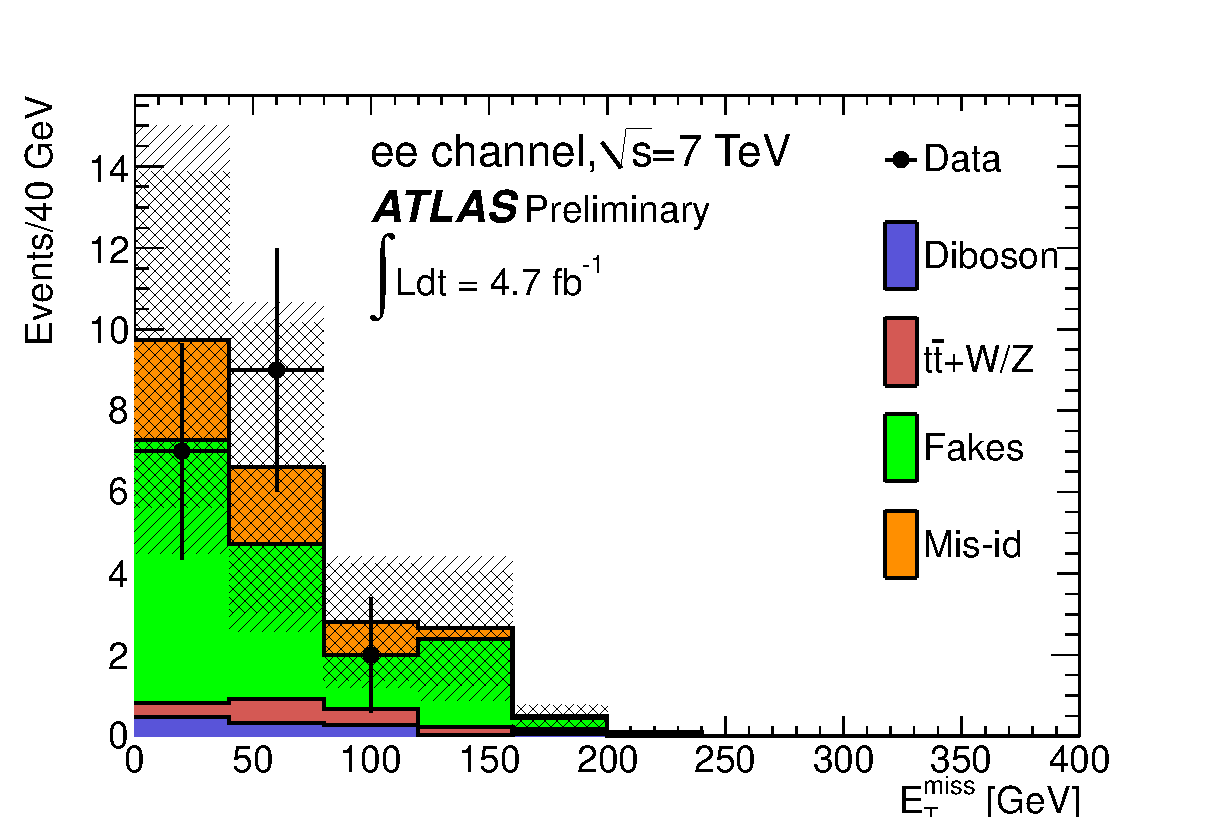
\includegraphics[scale=0.30]{figures/samesign/Signal/sig_nohtnomet_met_ee}}
\subfigure[\label{sig_ht_ee}]{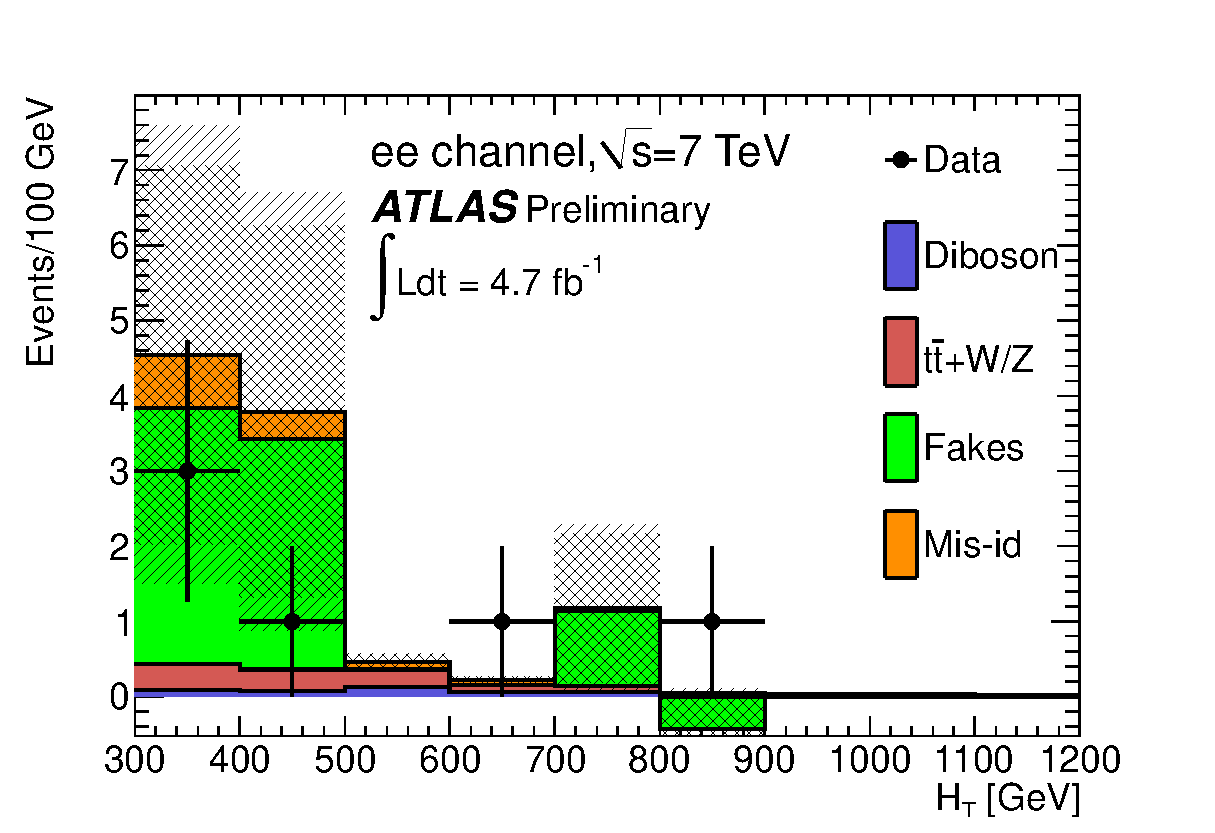
\includegraphics[scale=0.30]{figures/samesign/Signal/sig_noht_ht_ee}} \\
\subfigure[\label{sig_met_em}]{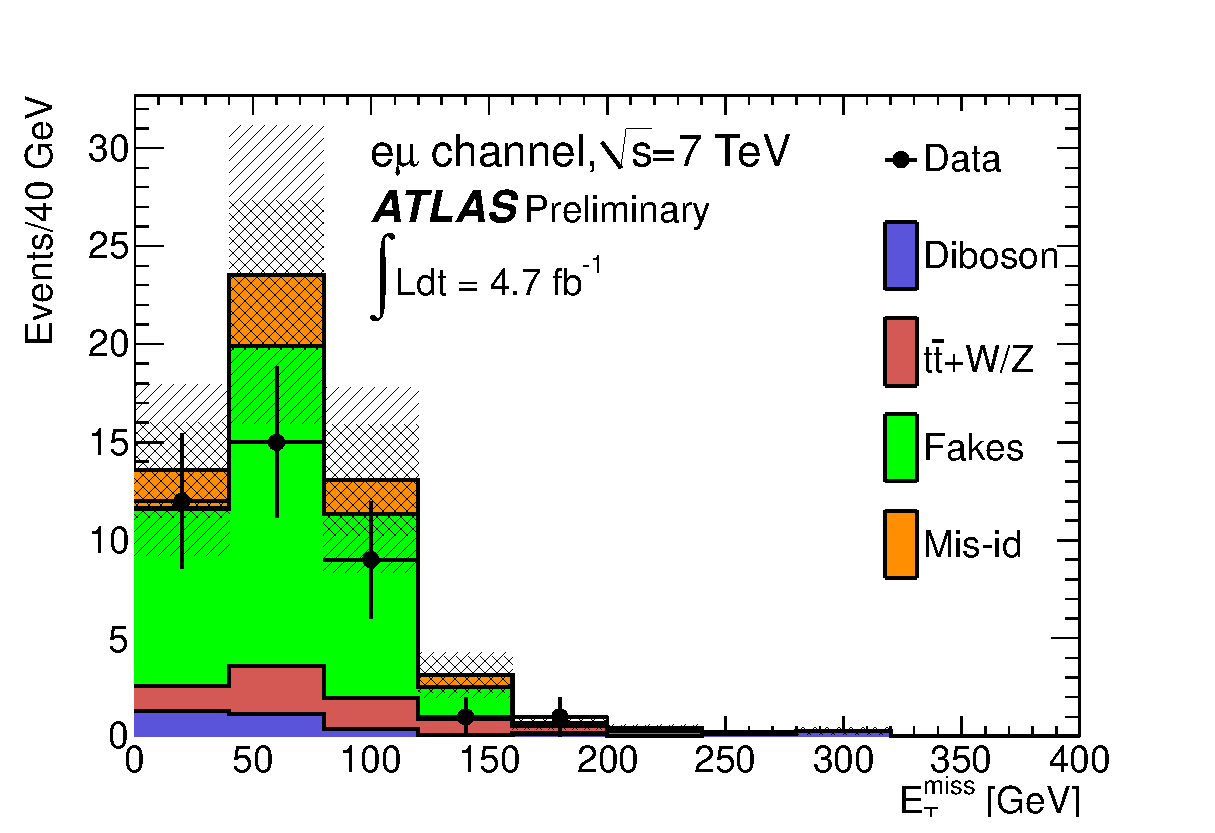
\includegraphics[scale=0.30]{figures/samesign/Signal/sig_nohtnomet_met_em}}
\subfigure[\label{sig_ht_em}]{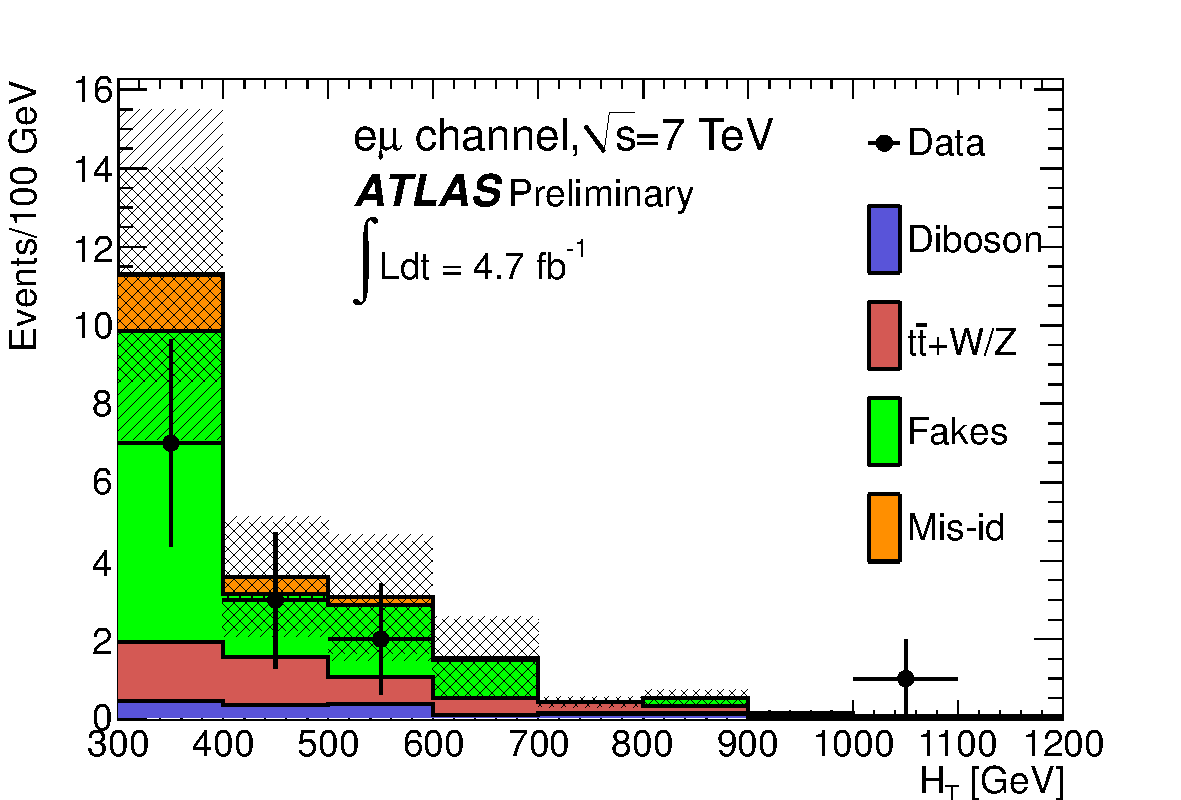
\includegraphics[scale=0.30]{figures/samesign/Signal/sig_noht_ht_em}} \\
\subfigure[\label{sig_met_mm}]{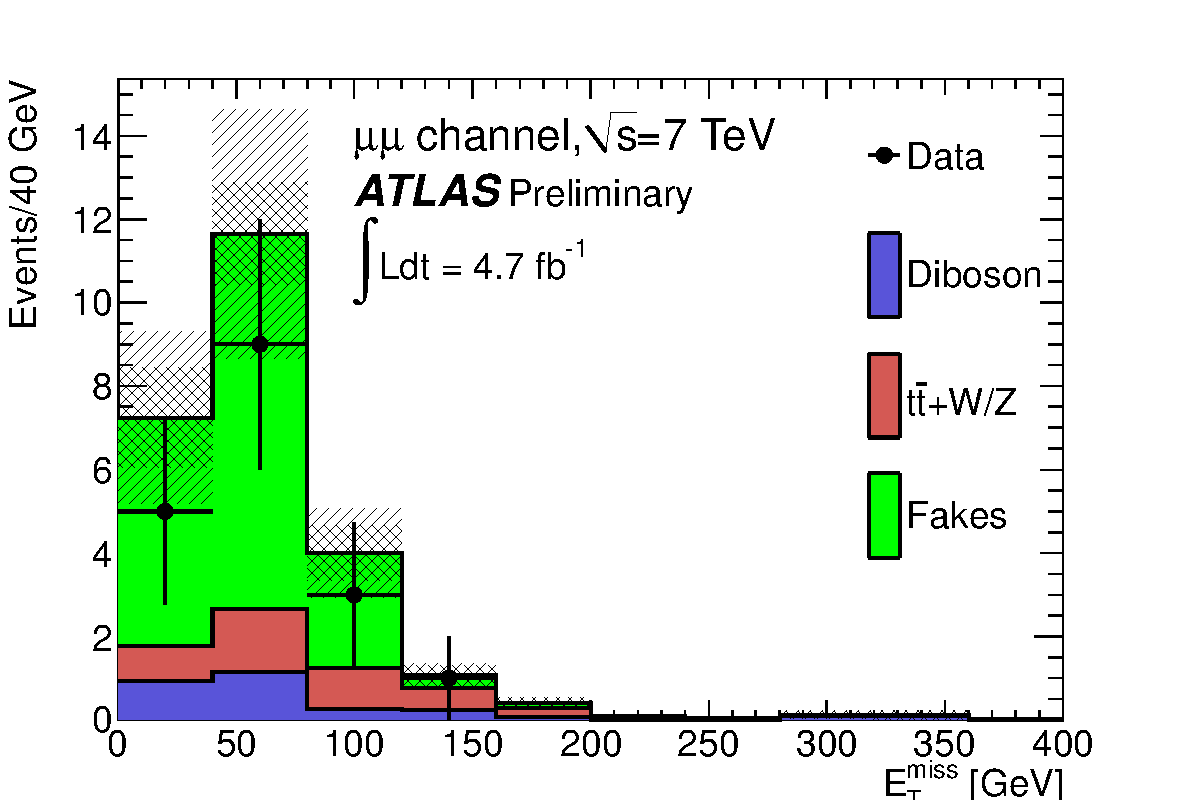
\includegraphics[scale=0.30]{figures/samesign/Signal/sig_nohtnomet_met_mm}}
\subfigure[\label{sig_ht_mm}]{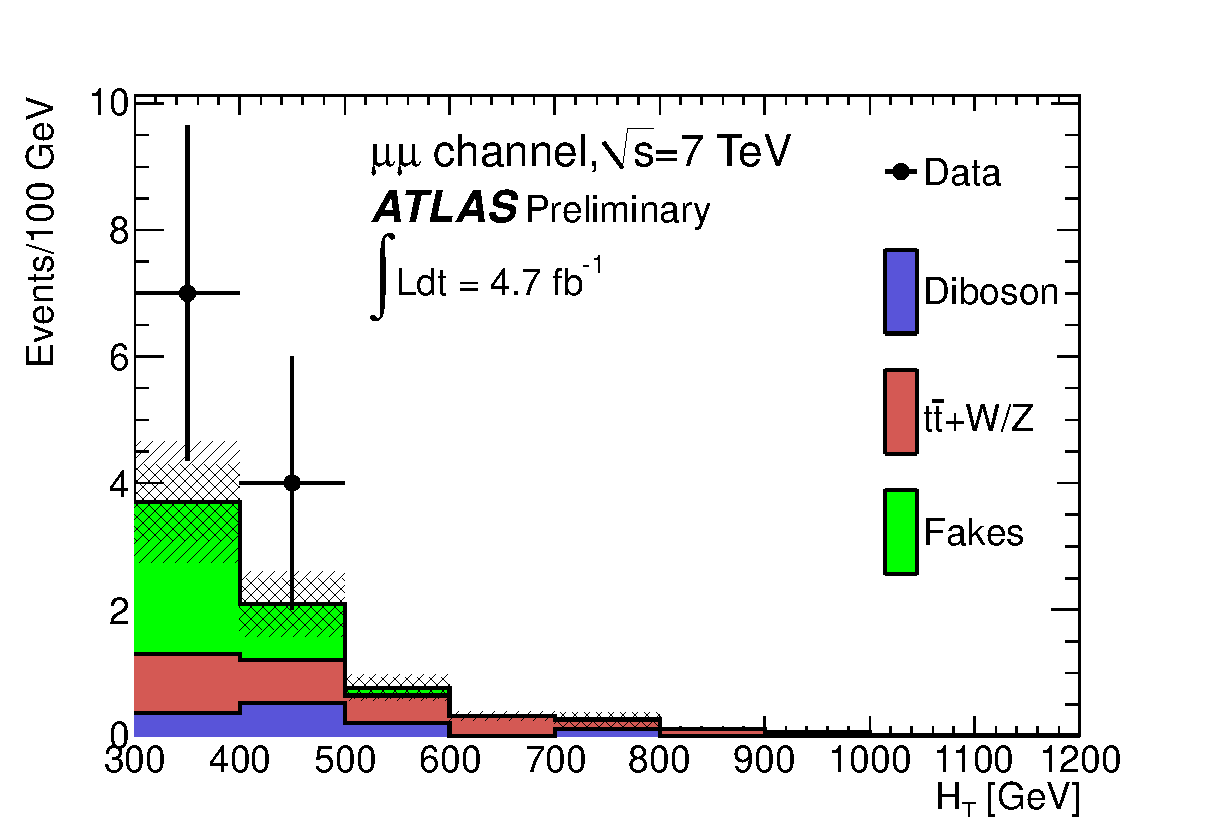
\includegraphics[scale=0.30]{figures/samesign/Signal/sig_noht_ht_mm}}
\caption{Distribution of \met{} for the data (points) and for the estimated background (histogram),after applying the signal selection except the cuts on \met{} and \HT{}, for the $ee$ (a), $e\mu$ (c)
and $\mu\mu$ (e) channels. Distribution of \HT{} after applying the selection except the \HT{} cut, for the $ee$ (b), $e\mu$ (d) and $\mu\mu$ (f) channels. The internal shaded areas correspond to the
statistical uncertainties on the background while the external shaded areas correspond to the total uncertainties. For the Monte Carlo samples, systematic uncertainties include only the production cross section uncertainties.}\label{fig:signal}
\end{figure}


%% \section{Results}\label{sect:results}
%% After applying the selection to the data, we find four events in the signal region, with $5.6\pm1.7$ 
%% expected background events. The details of the observed number of events are shown in 
%% Table~\ref{finalyield}, as well as the total expected number of background events. 
%% No significant excess is observed in the data, 
%% therefore limits on the signals are computed in the following section.

%% The distributions of the \met{} and \HT{} variables observed in data are compared to the background
%% estimates in Figure~\ref{fig:signal} and show a good agreement.

%% \begin{table}[t]
%%   \begin{center}
%%     \caption{Observed number of events and expected number of background events with 
%%         statistical (first) and systematic (second) uncertainties for the signal region
%%         selection.}\label{finalyield}
%%     \begin{tabular}{l|c|c|c}
%%       \hline\hline
%%        & \multicolumn{3}{c}{Channel} \\
%%       \cline{2-4}
%%       Backgrounds & $ee$ & $e\mu$ & $\mu\mu$ \\
%%       \hline
%%       Mis-id & $0.13\pm 0.04 \pm 0.02$ & $0.23\pm 0.04 \pm 0.03$ & --- \\
%%       Fakes & $0.5\pm 1.1 \pm 0.3$ & $0.8\pm 1.1 \pm 0.3$ & $0.13\pm 0.13\pm 0.04$ \\
%%       \hline
%%       Diboson & & & \\
%%       $\bullet$ $WZ/ZZ$+jets & $0.19\pm 0.20 \pm 0.07$ & $0.34\pm 0.21\pm 0.13$ & $0.28\pm 0.22\pm 0.10$ \\
%%       $\bullet$ $W^{\pm}W^\pm$+2 jets & $0.06\pm 0.03\pm 0.03$ & $0.07\pm 0.03\pm 0.03$ & $0.03\pm 0.02\pm 0.03$ \\
%%       \hline
%%       $t\bar{t}+W/Z$ & & & \\
%%       $\bullet$ $t\bar{t}W$(+jet) & $0.23\pm 0.02\pm 0.07$ & $0.79\pm 0.04\pm 0.24$ & $0.57\pm 0.04\pm 0.18$ \\
%%       $\bullet$ $t\bar{t}Z$(+jet) & $0.17\pm 0.02\pm 0.09$ & $0.61\pm 0.03\pm 0.31$ & $0.33\pm 0.02\pm 0.17$ \\
%%       $\bullet$ $t\bar{t}W^{\pm}W^\mp$ & $0.008\pm 0.001\pm 0.002$ & $0.023\pm 0.001\pm 0.007$ & $0.016\pm 0.001\pm 0.005$ \\
%%       \hline
%%       Total & $1.3 \pm 1.1 \pm 0.3$ & $2.9 \pm 1.1 \pm 0.5$ & $1.36 \pm 0.26 \pm 0.27$ \\
%%       \hline
%%       Observed & 2 & 2 & 0 \\
%%       \hline
%%     \end{tabular}
%%   \end{center}
%% \end{table}

%% \begin{figure}[t]
%% \centering
%% \subfigure[\label{sig_met_ee}]{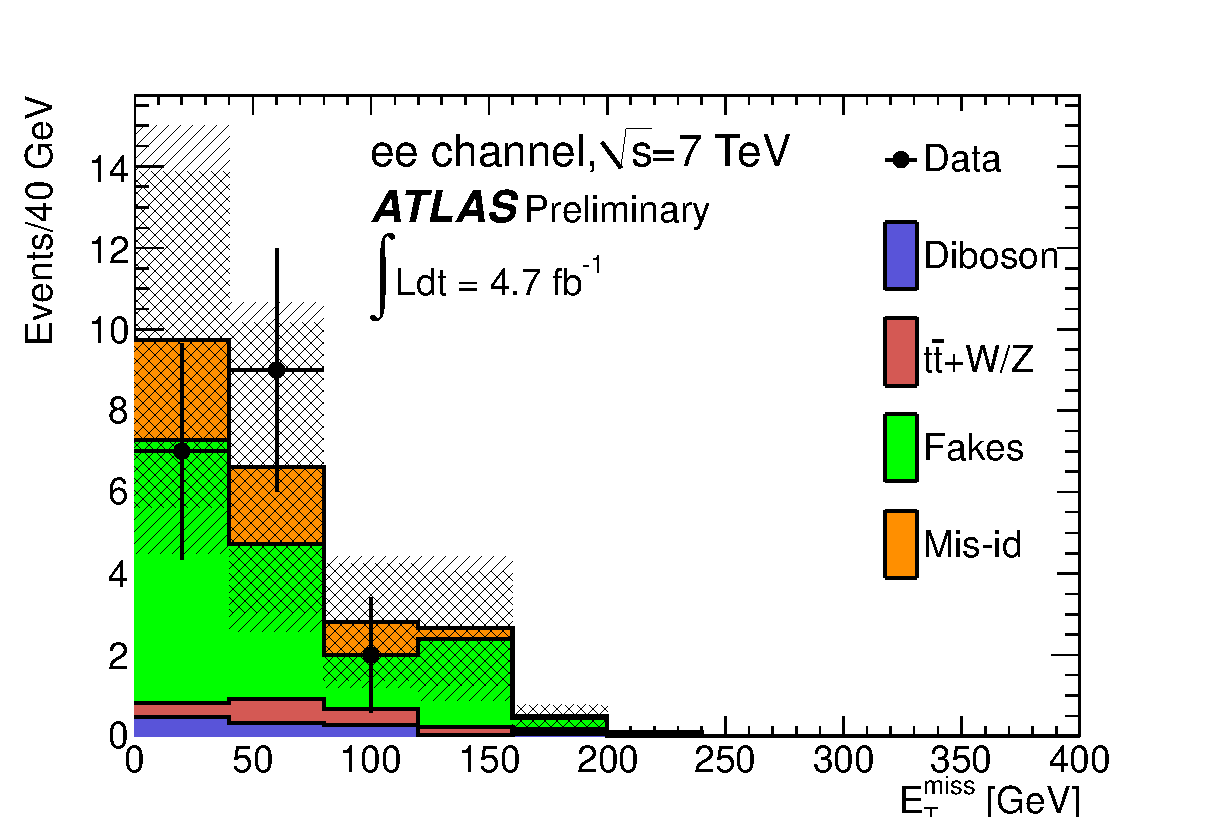
\includegraphics[scale=0.38]{figures/samesign/Signal/sig_nohtnomet_met_ee}}
%% \subfigure[\label{sig_ht_ee}]{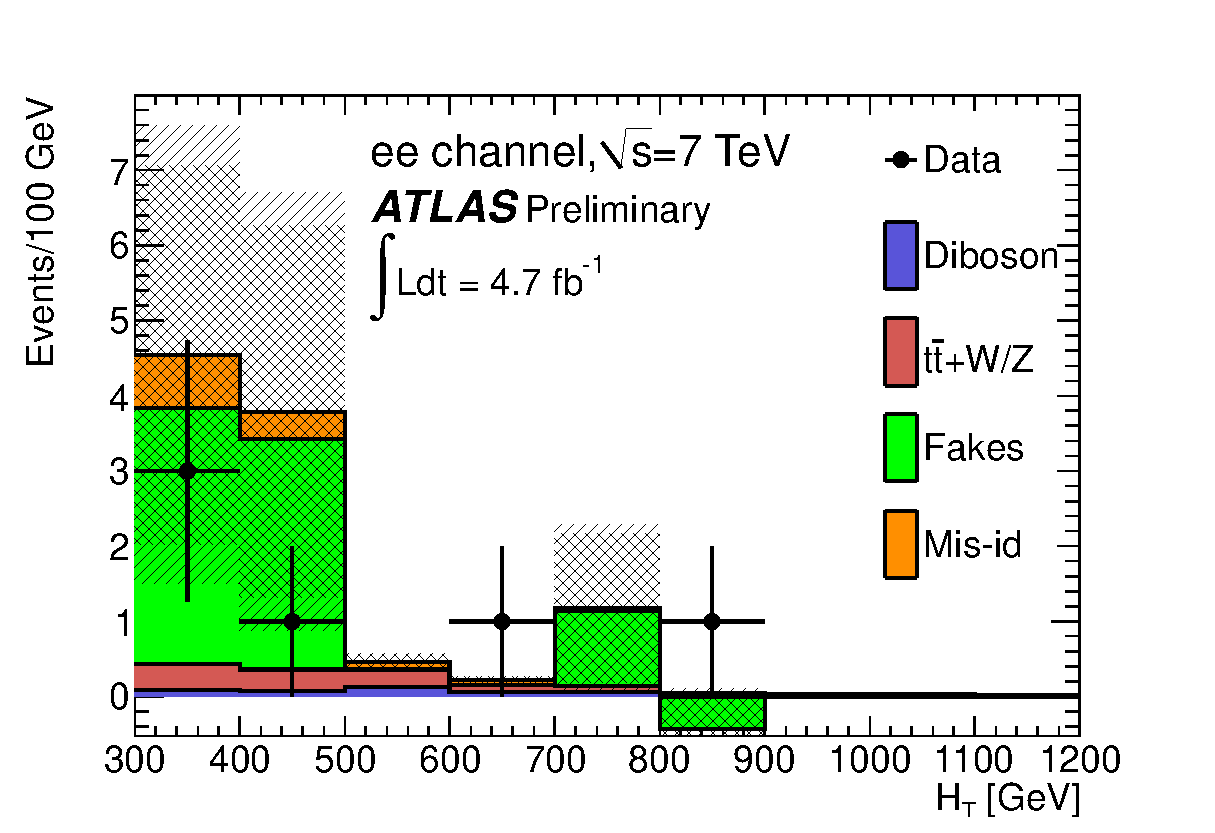
\includegraphics[scale=0.38]{figures/samesign/Signal/sig_noht_ht_ee}}
%% \subfigure[\label{sig_met_em}]{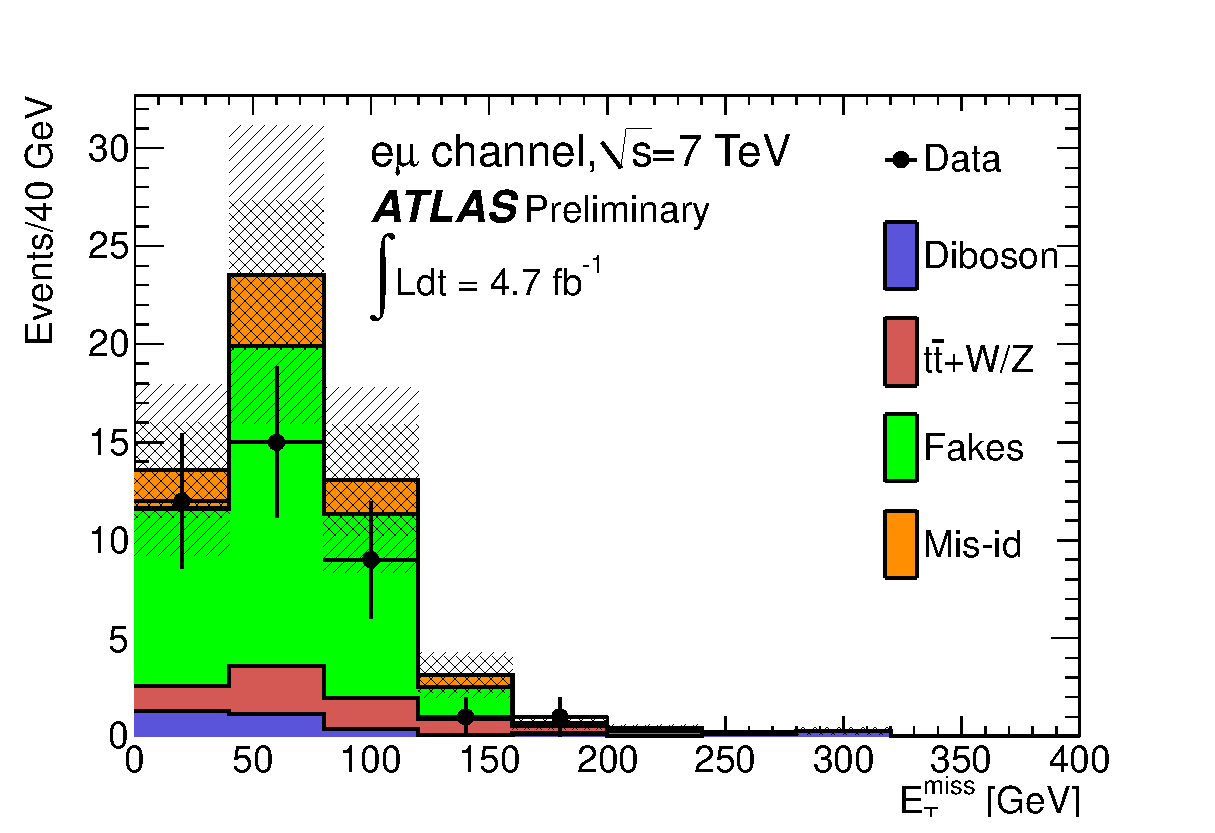
\includegraphics[scale=0.38]{figures/samesign/Signal/sig_nohtnomet_met_em}}
%% \subfigure[\label{sig_ht_em}]{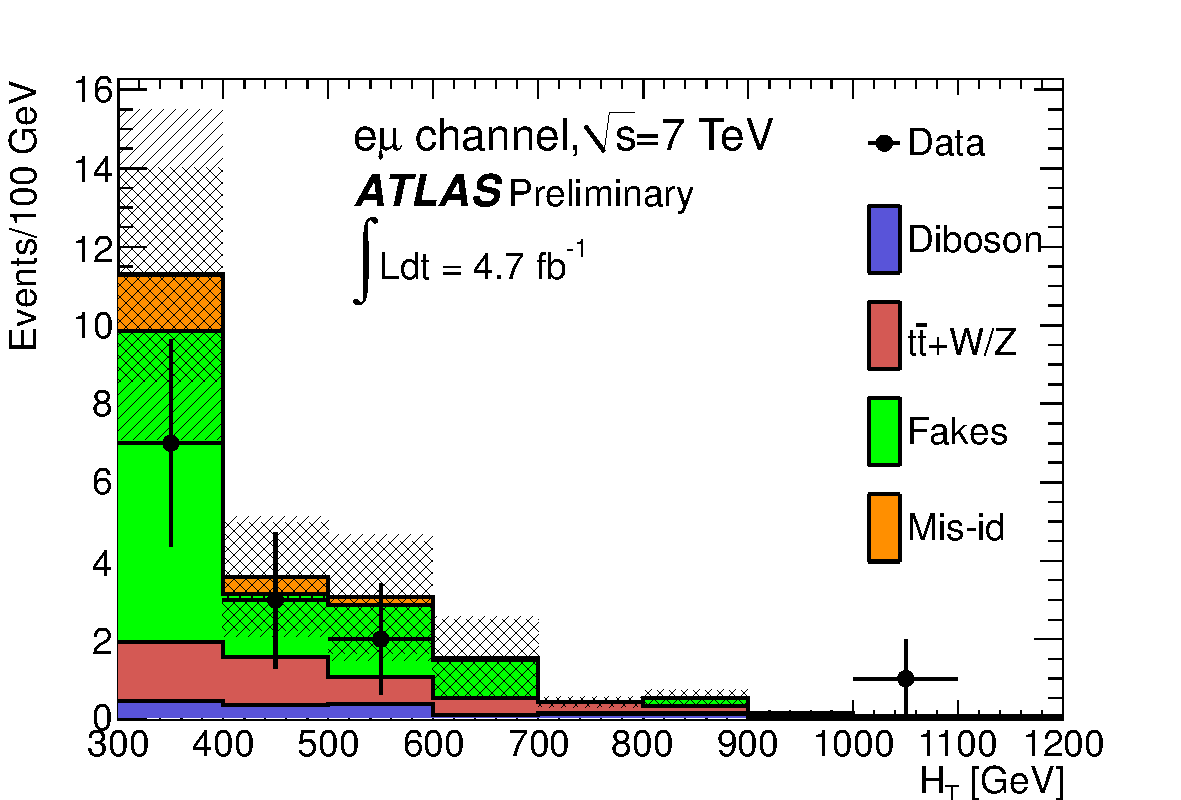
\includegraphics[scale=0.38]{figures/samesign/Signal/sig_noht_ht_em}}
%% \subfigure[\label{sig_met_mm}]{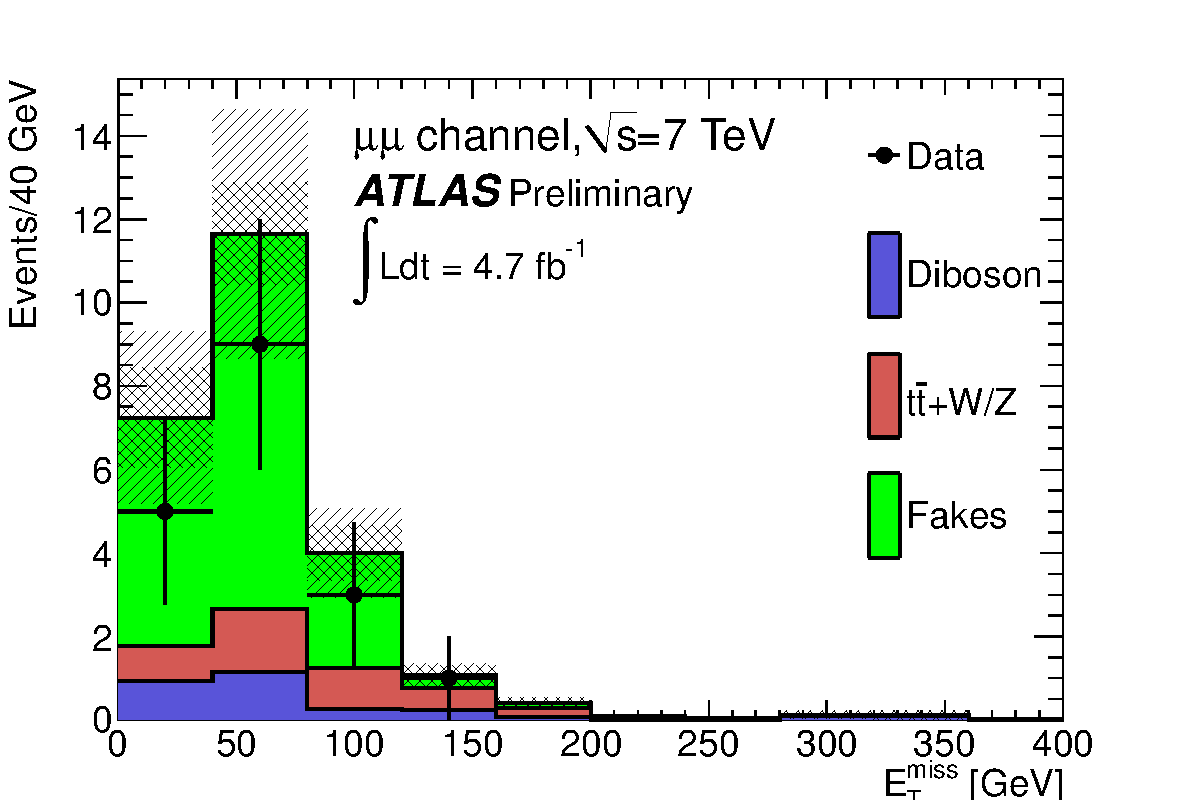
\includegraphics[scale=0.38]{figures/samesign/Signal/sig_nohtnomet_met_mm}}
%% \subfigure[\label{sig_ht_mm}]{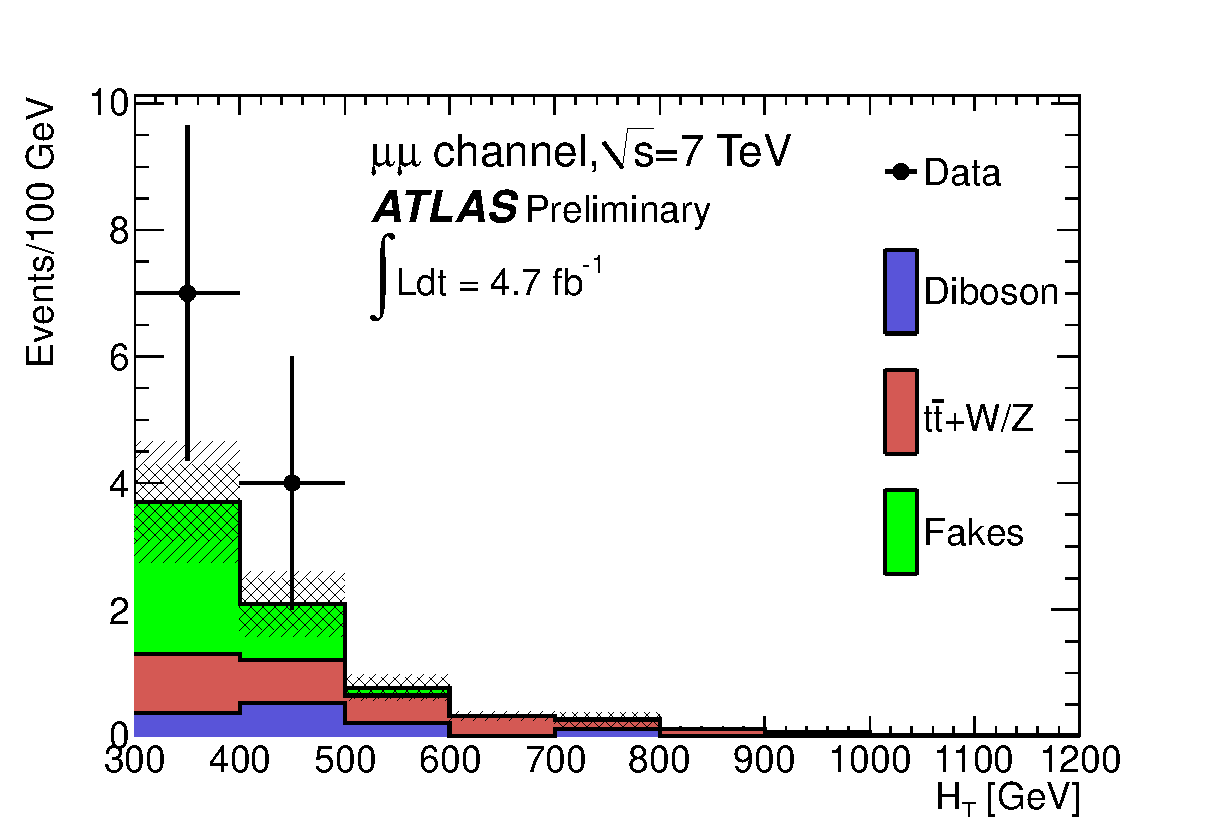
\includegraphics[scale=0.38]{figures/samesign/Signal/sig_noht_ht_mm}}
%% \caption{Distribution of \met{} for the data (points) and for the estimated background (histogram),
%% after applying the signal selection except the cuts on \met{} and \HT{}, for the $ee$ (a), $e\mu$ (c)
%% and $\mu\mu$ (e) channels. Distribution of \HT{} after applying the selection except the \HT{} cut,
%% for the $ee$ (b), $e\mu$ (d) and $\mu\mu$ (f) channels. The internal shaded areas correspond to the
%% statistical uncertainties on the background while the external shaded areas correspond to the total
%% uncertainties. For the Monte Carlo samples, systematic uncertainties include only the production 
%% cross section uncertainties.}\label{fig:signal}
%% \end{figure}

\clearpage
\section{Interpretation of the results}\label{sect:interpretation}

Each model is studied using a likelihood function that models the number of expected events in the three signal regions, including the presents of both signal and background and the effect of systematic uncertainties.
For models that include the mass of a particle as a free parameter, several likelihood functions are constructed, each built to model a specific mass point.
Parameters representing the total cross-section of each signal process at each mass point are included in the likelihood function, and statistical tests are run to place limits on the size of these parameters.
For each model studied, upper limits at 95\% C.L. on the cross sections of the hypothetical processes are derived using the $CL_S$ method~\cite{Junk:1999kv,0954-3899-28-10-313}.
Systematic uncertainties enter the likelihood as parameters constrained by gaussian distributions which allow the expected number of signal or background events to fluctuate upwards or downwards coherently across the three signal regions.

%% \section{Interpretation of the results}\label{sect:interpretation}
%% For each model, upper limits at 95\% C.L. on the cross sections of the hypothetical
%% processes are derived using the $CL_S$ method~\cite{Junk:1999kv,0954-3899-28-10-313}. We use
%% single-bin counting experiments to extract the most likely signal cross section.
%% Systematic uncertainties are included as variations in the expected signal and background
%% yields, which are allowed to vary in the ensembles used to generate the $CL_S$ distributions.
%% Correlations of the systematic uncertainties across samples and channels are taken into account. 
%% It must also be noted that each sample is statistically varied independently, using a Gaussian function
%% truncated at zero\footnote{A cross-check was done replacing the truncated Gaussian function by a 
%% log-normal distribution and the results are very similar.}, in order to avoid negative contributions, 
%% in particular for the samples which have a very low yield and a large statistical uncertainty.


The 95\% C.L. upper limits on the production cross sections of a pair of $b^\prime$ or $T_{5/3}$ are extracted for each hypothesis of mass of the new particle.
A model is considered to be excluded when the 95\% confidence limit on the upper limit of the cross-section is less than the model's nominal cross-section.
Comparing these limits to the predicted cross section as a function of the mass, as can be seen in Figure~\ref{limit:bprime}, we set a lower limit of 0.67~\TeV{} on the mass of the $b^\prime$ quark and of the $T_{5/3}$ in the case $\lambda\ll1$, with an expected limit of 0.64~\TeV{}.

%% \section{Pair production of $b^\prime$ and $T_{5/3}$}
%% The 95\% C.L. upper limits on the production cross sections of a pair of $b^\prime$ or $T_{5/3}$ 
%% are extracted
%% for each hypothesis of mass of the new particle. Comparing these limits to the predicted cross section
%% as a function of the mass, as can be seen in Figure~\ref{limit:bprime}, we set a lower limit of 
%% 0.67~\TeV{} on the mass of the $b^\prime$ quark and of the $T_{5/3}$ in the case $\lambda\ll1$, with an
%% expected limit of 0.64~\TeV{}.

\begin{figure}[t]  
  \begin{center}
    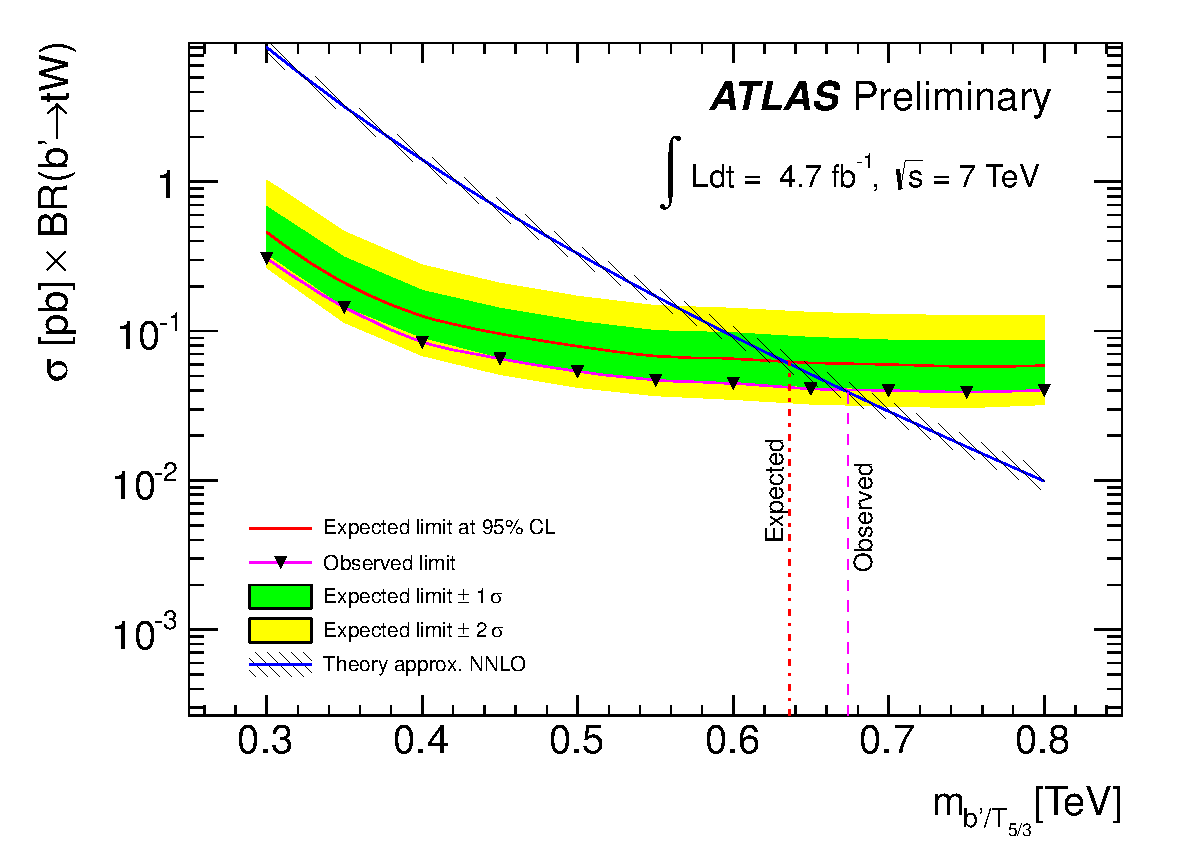
\includegraphics[width=0.8\textwidth]{figures/samesign/Limit_bprime_final_obs_CS}
    \caption{Expected and observed upper limits on the pair production cross section 
        of the $b^\prime$ and $T_{5/3}$, as a function of their mass.}
    \label{limit:bprime}

    \vspace{1cm}

    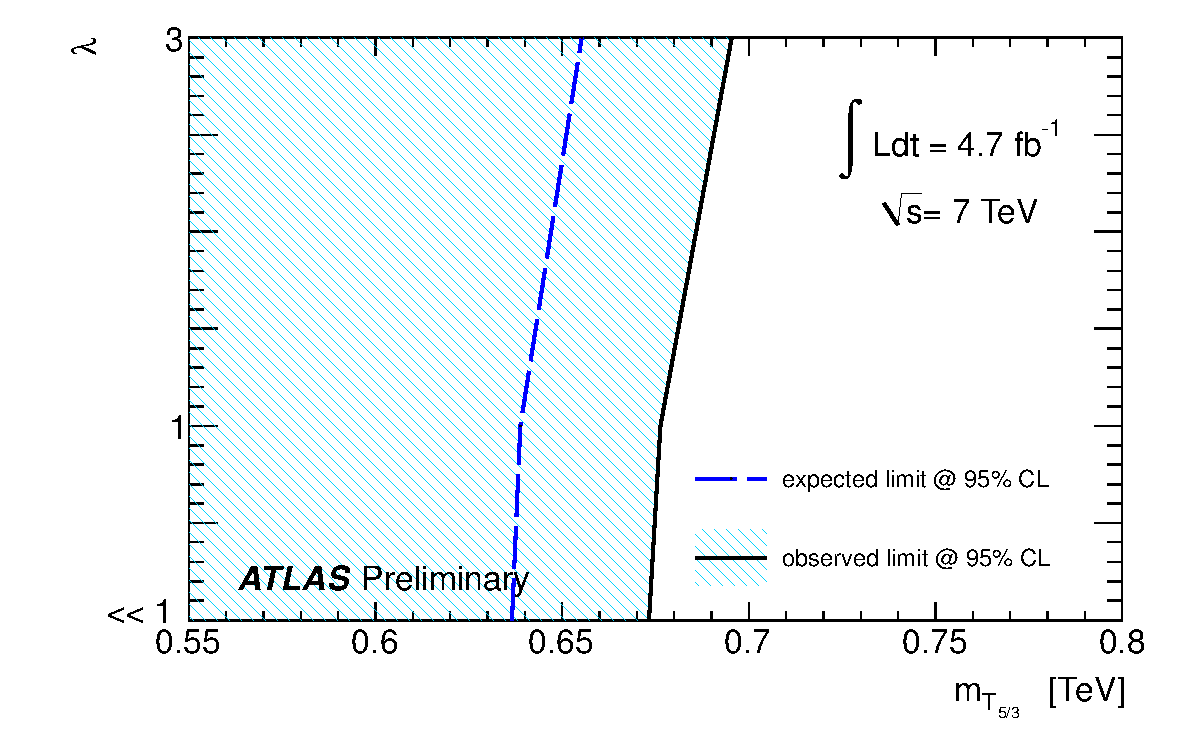
\includegraphics[width=0.8\textwidth]{figures/samesign/limit_observed_T53}
    \caption{Expected and observed lower limits on the $T_{5/3}$ signal, as a function 
        of the $T_{5/3}$ mass and the coupling constant $\lambda$. The shaded area  is excluded 
        at 95\% C.L.}
    \label{limit:t53}
  \end{center}
\end{figure}


\section{Single and pair production of the $T_{5/3}$}

Contributions from both the single and pair production of $T_{5/3}$ are included when the coupling constants  $\lambda=1$ and $\lambda=3$ are studied.
The 95\% C.L. upper limits on the production cross sections are used to derive lower limits on the mass of the $T_{5/3}$ at 0.68~\TeV{} for $\lambda=1$ and 0.70~\TeV{} for $\lambda=3$, with expected limits of 0.64~\TeV{} and 0.66~\TeV{}, respectively. 
These results, combined with the pair production result, are summarized in Figure~\ref{limit:t53}.

%% \section{Single and pair production of the $T_{5/3}$}
%% For the two cases $\lambda=1$ and $\lambda=3$, both the single and pair production of the $T_{5/3}$
%% must be included. The 95\% C.L. upper limits on the production cross sections are used to
%% derive lower limits on the mass of the $T_{5/3}$ at 0.68~\TeV{} for $\lambda=1$ and 0.70~\TeV{} for
%% $\lambda=3$, with expected limits of 0.64~\TeV{} and 0.66~\TeV{}, respectively. These results, combined with
%% the pair production result, are summarized in Figure~\ref{limit:t53}.


\section{Four top quarks production}

An upper limit at 95\% C.L. of 61~fb is derived for the production cross section of four top quarks events through a contact interaction, with an expected limit of 90~fb.
%Because the final state produced by this model is kinematically similar to the four-tops final state produced in the Standard Model, this result can be used to place an approximate limit on the Standard
This result can be used as a benchmark of comparison for other models that lead to four-top interactions provided that the kinematics of their final states are comparable.


%This result can be extrapolated to other models, as long as the kinematical properties of the produced events are similar to the ones generated by the four-top quark contact interaction. 
%In particular, a study at parton level of SM four-top quark events has shown that the global acceptance of this SM signal is only about 15\% lower than the acceptance for the four top quarks signal considered in this analysis. 
%Therefore, one can set an upper limit on the SM four top quarks production of the same order of magnitude.

%% \section{Four top quarks production}
%% An upper limit
%% at 95\% C.L. of 61~fb is derived for the production cross section of four top quarks events
%% through a contact interaction, with an expected limit of 90~fb.
%% This result can be extrapolated to other models, as long as the kinematical properties of the 
%% produced events are similar to the ones generated by the four-top quark contact interaction. In
%% particular, a study at parton level of SM four-top quark events has shown that the
%% global acceptance of this SM signal is only about 15\% lower than the acceptance
%% for the four top quarks signal considered in this analysis. Therefore, one can set an upper limit on the
%% SM four top quarks production of the same order of magnitude.

\section{Conclusion}\label{sect:conclusion}

This section described a search for exotic processes in the same-sign dilepton plus jets signature with the ATLAS detector at LHC at $\sqrt{s}=7 \TeV$.
The searched used the full 2011 ATLAS $pp$ dataset, and selected events by requiring at least two jets, including at least one $b$-tagged jet, $\met>40 \GeV$ and $\HT>550 \GeV$, where \HT{} denotes the scalar sum of the \pT{} of all leptons and jets. 

Four events have been observed in this signal region with an expected background of $5.6\pm1.7$ events. 
This result has been interpreted in terms of several new physics models, including the pair production of down-type heavy quarks ($b^\prime$), the single and pair production of heavy quark partners ($T_{5/3}$), and the production of events containing four top quarks through a four-top quark contact interaction. 
The various limits which have been set are summarized in Table~\ref{limit:all}.

%% \section{Conclusion}\label{sect:conclusion}
%% In conclusion, a search for exotic processes in the same-sign dilepton plus jets signature with the
%% ATLAS detector at LHC at $\sqrt{s}=7 \TeV$
%% has been presented. The events are selected by requiring at least two jets, including at
%% least one $b$-tagged jet, $\met>40 \GeV$ and $\HT>550 \GeV$, with \HT{} being the scalar sum of the \pT{}
%% of all leptons and jets. The full 2011 ATLAS $pp$ dataset,
%% corresponding to 4.7~\ifb{}, was used in this search. Four events have been observed with an expected
%% background of $5.6\pm1.7$ events. This result has been interpreted in terms of the pair production 
%% of down-type heavy quarks ($b^\prime$), the single and pair production of heavy quark partners
%% ($T_{5/3}$), and the production of events containing four top quarks through a four-top quark
%% contact interaction. The various limits which have been set are summarized in Table~\ref{limit:all}.

%% The obtained limit on the $b^\prime$ and $T_{5/3}$ mass in the pair production is the most stringent 
%% limit to date in the same-sign dilepton channel. The limits obtained on the $T_{5/3}$ including the
%% single production, and on four top quark event production are the first results on these signals.


\begin{table}[t]
  \begin{center}
    \caption{Expected and observed limits on the masses of the $b^\prime$ and $T_{5/3}$
        and on the four top quark events production cross-section.}\label{limit:all}
    \begin{tabular}{l|c|c}
      \hline\hline
      & \multicolumn{2}{c}{95\% C.L. limits} \\
      \cline{2-3}
      Constrained parameter & Expected & Observed \\
      \hline
      \multicolumn{3}{c}{$b^\prime$ / $T_{5/3}$ pair production} \\
      \hline
      $b^\prime$ mass or $T_{5/3}$ mass for $\lambda\ll1$ & $>0.64 \TeV$ & $>0.67 \TeV$ \\
      \hline
      \multicolumn{3}{c}{$T_{5/3}$ single and pair production} \\
      \hline
      $T_{5/3}$ mass for $\lambda=1$ & $>0.64 \TeV$ & $>0.68 \TeV$ \\
      $T_{5/3}$ mass for $\lambda=3$ & $>0.66 \TeV$ & $>0.70 \TeV$ \\
      \hline
      \multicolumn{3}{c}{Four top quark event production} \\
      \hline
       Four top quark production cross-section & $<90$ fb & $<61$ fb \\
      \hline
    \end{tabular}
  \end{center}
\end{table}
